\documentclass[11pt]{report}
\setlength\parindent{24pt}
\usepackage[a4paper]{geometry}
\geometry{top=2cm, bottom=2cm, left=3cm, right=2cm}
\usepackage{tikz}
\usepackage{pgfplots}
\pgfplotsset{compat = newest}
\usepackage{parskip}
\usepackage{subcaption}
\usepackage{array}
\usepackage{amsmath}
\usepackage{amssymb}
\usepackage{tabularcalc}
\usetikzlibrary{math,angles,quotes}
\usepackage{siunitx}
\usepackage{tkz-euclide}
\usepackage{wrapfig}
\usepackage{cancel}
\usepackage{multirow}
\usepackage{multicol}
\usepackage{blindtext}

\newcommand{\R}{\mathbb{R}}
\newcommand{\dx}{\frac{d}{dx}}
\newcommand{\dt}{\frac{d}{dt}}


\begin{document}
%-----------------------------------PORTADA------------------------------------%------------------------------------------------------------------------------
\null
\vfill
\begin{figure}[h]
\centering

\includegraphics[width=8cm, height=11cm]{logo}\\[10mm]
{\LARGE\textbf{Universidad de Guadalajara}}\\[2mm]
Centro Universitario de la Costa\\[2mm]
\textit{Trabajo final de Seminario de Solucion de Problemas de Métodos Matemáticos I} \\[2mm]
Alumno: Nemesis Jessiel Sierra Aranda\\[2mm]
Código de alumno: 221404306\\[2mm]
Profesor: Jahaziel Méndez García\\[2mm]
28/06/2021\\
\end{figure}
\vfill
%-------------------------NUMEROS REALES Y COMPLEJOS---------------------------%------------------------------------------------------------------------------
\pagebreak \textbf {Números reales y complejos}\\[2mm]
a) Resolver los siguientes ejercicios de números complejos:\\[2mm]
\indent {1) $(3+2i)+(6-4i)$}\\[2mm]
\indent Resolviendo:

$$(3+6)+(2i-4i)$$
$$9+(2i-4i)$$
$$9-2i$$

\indent {2) $(3-5i)-(1-3i)$}\\[2mm]
\indent Resolviendo:

$$(3+1)-(-5i-3i)$$
$$4-(-8i)$$
$$4+8i$$

\indent {3) $(2-4i)(3-2i)$}\\[2mm]
\indent Resolviendo:

$$(2)(3-2i)-4i(3-2i)$$
$$6-4i-4i(3-2i)$$
$$6-4i-12i+8i^2$$

\indent Recordando que $i^2=-1$ entonces:

$$6-4i-12i+8(-1)$$
$$6-4i-12i-8$$
$$-2-16i$$

%-----------------------------ECUACIONES CUADRATICAS---------------------------%------------------------------------------------------------------------------
\pagebreak \textbf {Ecuaciones cuadráticas}\\[2mm]
Resolver los siguientes ejercicios de ecuaciones cuadráticas.\\[2mm]
a) Por factorización:\\[2mm]
\indent \textbf {1) $4u^2-8u$}\\[2mm]
\indent Igualar a cero primero y ordenar

$$4u^2-8u=0$$

\indent La forma de factorización es

$$ax^2-x+a=0$$
$$\frac{4u^{2}-8u}{4}$$
$$\frac{16u^{2}-32u}{4}$$
$$\frac{(4u)^{2}-4(8u)}{4}$$

\indent Factorizo el cociente

$$\frac { (4u-4)(4u+0) } {4}$$
$$(u-2)(u)=0$$

\indent Donde $(u-2)$ corresponde a nuestra primer raíz y $(u)$ a la segunda, por lo tanto:

$$u_1=2$$ $$u_2=0$$

\indent \textbf {2) $2d^{2}+15d=8$}\\[2mm]
\indent Igualamos a cero y ordenamos la ecuación

$$2d^{2}+15d-8=0$$

\indent Hacemos la factorización

$$(x+8)(2x-1)=0$$

\indent Por lo que sus raíces serán $x+8=0$ y $2x-1=0$

$$x_1+8=0$$
$$x_1=-8$$
$$2x_2-1=0$$
$$2x_2=1$$
$$x_2=\frac{1}{2}$$

\indent \textbf {3) $2x^{2}+12=11x$}\\[2mm]
\indent Ordenamos e igualamos a cero

$$2x^{2}-11x+12=0$$

\indent Factorizamos en dos términos

$$(x-4)(2x-3)=0$$
$$x_1-4=0$$
$$x_1=4$$
$$2x_2-3=0$$
$$2x_2=3$$
$$x_2=\frac{3}{2}$$

a) Por raíz cuadrada:\\[2mm]
\indent \textbf { 1) $x^{2}-25=0$ }

$$x^{2}=25$$
$$\sqrt {x^{2}}=\sqrt{ 25 }$$
$$x_1=5$$ $$x_2=-5$$

\indent \textbf { 2) $x^{2}+16=0$ }

$$x^{2}=-16$$
$$\sqrt{ x^{2} }=\sqrt{ -16 } $$
$$x_1=-4i$$ $$x_2=4i$$

\indent \textbf { 3) $9y^{2}-16=0$ }

$$9y^{2}=16$$
$$\sqrt{ 9y^{2} }=\sqrt{16}$$
$$3y=4$$
$$y_1=\frac{4}{3}$$ $$y_2=-\frac{4}{3}$$

\pagebreak b) Por fórmula cuadrática:\\[2mm]
\indent \textbf { 1) $x^{2}-10x-3=0$ }\\[2mm]
\indent Utilizando la formula general:

$$x=\frac{ -b\pm \sqrt{ b^{2}-4(a)(c) } }{ 2(a) }$$

\indent Obtenemos:

$$x=\frac{ -(-10)\pm \sqrt{ (-10)^{2}-4(-3) } }{ 2 }$$
$$x=\frac{ 10\pm \sqrt{ 100+12 } }{ 2 }$$
$$x=\frac{ 10\pm \sqrt{ 112 } }{ 2 }$$
$$x=\frac{ 10\pm \sqrt{ 16\cdot7 } }{ 2 }$$
$$x=\frac{ 10\pm \sqrt{ 2^{4}\cdot7 } }{ 2 }$$
$$x=\frac{ 10\pm \sqrt{ 2^{4}}\cdot\sqrt{7 } }{ 2 }$$
$$x_1=\frac{ 10+4\sqrt{7 } }{ 2 }$$
$$x_2=\frac{ 10-4\sqrt{7 } }{ 2 }$$

\indent Factorizamos $2$ de $10+4\sqrt{7}$ obtenemos $2(2\sqrt{7}+5)$ entonces:

$$x_1=\frac{ 2(2\sqrt{ 7 }+5) }{ 2 }$$
$$x_1=5+2\sqrt{7}$$

\indent Factorizamos $2$ de $10-4\sqrt{7}$ obtenemos $2(-2\sqrt{7}+5)$ entonces:

$$x_2=\frac{ 2(-2\sqrt{ 7 }+5) }{ 2 }$$
$$x_2=5-2\sqrt{7}$$

\indent \textbf { 2) $t^{2}=1-t$ }\\[2mm]
\indent Ordenamos e igualamos a cero:

$$t^{2}+t-1=0$$

\indent Aplicamos la fórmula general:

$$x=\frac{ -1\pm \sqrt{ (1)^{2}-4(-1) } }{ 2 }$$
$$x=\frac{ -1\pm \sqrt{ 1+4 } }{ 2 }$$
$$x=\frac{ -1\pm \sqrt{ 5 } }{ 2 }$$
$$x_1=-\frac{1}{2}+\frac{\sqrt{5}}{2}$$ $$x_2=-\frac{1}{2}-\frac{\sqrt{5}}{2}$$

\indent \textbf {3) $x^{2}+8=4x$ }\\[2mm]
\indent Ordenamos:

$$x^{2}-4x+8=0$$

\indent Resolvemos con la fórmula general:

$$x=\frac{ -(-4)\pm \sqrt{(-4)^{2}-4(8)} }{ 2 }$$
$$x=\frac{4 \pm \sqrt{16-32}}{2}$$
$$\frac{4 \pm \sqrt{-16}}{2}$$
$$x_1=\frac{4+(-4i)}{2}$$
$$x_1=2-2i$$
$$x_2=\frac{4-(-4i)}{2}$$
$$x_2=2+2i$$

c) Completando el cuadrado:\\[2mm]
\indent \textbf { 1) $x^{2}-6x-3=0$ }\\[2mm]
\indent Separamos el 3

$$x^{2}-6x=3$$

\indent Para poder realizar la factorización sumo 9 de cada lado:

$$x^{2}-6x(+9)=3(+9)$$
$$x^{2}-6x+9=12$$

\indent Factorizo la ecuación:

$$(x+(-3))(x-(-3))=12$$
$$(x-3)(x+3)=12$$
$$(x-3)^{2}=12$$

\indent Saco las raíces de ambos lados para eliminar el cuadrado:

$$\sqrt{(x-3)^{2}}=\sqrt{12}$$
$$x-3=\pm 2\sqrt{3}$$
$$x_1=3+2\sqrt{3}$$
$$x_2=3-2\sqrt{3}$$

\indent \textbf { 2) $2y^{2}-6y+3=0$ }\\[2mm]
\indent Eliminamos el $2$ de $y^2$

$$\frac{2y^{2}-6y+3}{2}$$
$$y^{2}-3y+\frac{3}{2}=0$$

\indent pasamos el $\frac{3}{2}$ del otro lado de la operación:

$$y^{2}-3y=-\frac{3}{2}$$

\indent Sumo $\frac{9}{4}$ en ambos lados para realizar la factorización:

$$y^{2}-3y+\frac{9}{4}=\frac{3}{4}$$
$$\left(y-\frac{3}{2}\right)^{2}=\frac{3}{4}$$

\indent Eliminamos el cuadrado con las raices:

$$\sqrt{\left(y-\frac{3}{2}\right)^{2}}=\sqrt{\frac{3}{4}}$$
$$y-\frac{3}{2}=\pm \frac{\sqrt{3}}{2}$$
$$y=\frac{3}{2}\pm \frac{\sqrt{3}}{2}$$
$$y_1=\frac{3}{2}+\frac{\sqrt{3}}{2}$$
$$y_2=\frac{3}{2}-\frac{\sqrt{3}}{2}$$

\indent \textbf { 3) $3x^{2}-2x-2=0$ }\\[2mm]
\indent Eliminamos el $3$ de $x^2$

$$\frac{3x^{2}-2x-2}{3}$$
$$y^2-\frac{2x}{3}-\frac{2}{3}$$

\indent pasamos el $\frac{2}{3}$ del otro lado de la operación:

$$y^2-\frac{2x}{3}=\frac{2}{3}$$

\indent Sumo $\frac{1}{9}$ en ambos lados para realizar la factorización:

$$y^2-\frac{2x}{3}+\frac{1}{9}=\frac{7}{9}$$
$$\left(x-\frac{1}{3}\right)^2=\frac{7}{9}$$

\indent Eliminamos el cuadrado con las raices:

$$\sqrt{\left(x-\frac{1}{3}\right)^2}=\sqrt{\frac{7}{9}}$$
$$x-\frac{1}{3}=\frac{\sqrt{7}}{9}$$
$$x_1=\frac{1}{3}+\frac{\sqrt{7}}{9}$$
$$x_2=\frac{1}{3}-\frac{\sqrt{7}}{9}$$

%-----------------------------DIVISION SINTETICA-------------------------------%------------------------------------------------------------------------------
\pagebreak \textbf {División Sintética}\\[2mm]
\indent \textbf { 1) $(3x^{4}-x-4) \div (x+1)$ }\\[2mm]
\indent Debido a que $(x+1)$ es $x=-1$ el denominador termina siendo $-1$ \\[2mm]
\indent Dibujamos la tabla para realizar la división:

\begin{center}
	\begin{tabular}{c|ccccc|}
		$\div$& $x^{4}$ & $x^{3}$ & $x^{2}$ & $x$ & $i$\\ \hline
		& & & & &\\
		& & & & &\\
		-1 & & & & &\\ \hline
		& & & & & \\
	\end{tabular}
\end{center}

\indent donde $x^{4}$, $x^{3}$, $x^{2}$, $x$, y $i$ corresponden a los valores respectivos de la ecuación $(3x^{4}-x-4)$
\begin{center}
	\begin{tabular}{c|ccccc|}
		$\div$& $x^{4}$ & $x^{3}$ & $x^{2}$ & $x$ & $i$\\ \hline
		& 3 & 0 & 0 & -1 & -4\\
		& & & & &\\
		-1 & &  &  &  &  \\ \hline
		&  &  &  &  &  \\
	\end{tabular}
\end{center}

\indent Primero bajamos el $3$:
\begin{center}
	\begin{tabular}{c|ccccc|}
		$\div$& $x^{4}$ & $x^{3}$ & $x^{2}$ & $x$ & $i$\\ \hline
		& 3 & 0 & 0 & -1 & -4\\
		& & & & &\\
		-1 & &  &  &  &  \\ \hline
		& 3 &  &  &  & \\
	\end{tabular}
\end{center}

\indent El numero $3$ se divide por el denominador $-1$, se escribe el resultado en la siguiente columna \indent y se suma con el cero de arriba:
\begin{center}
	\begin{tabular}{c|ccccc|}
		$\div$& $x^{4}$ & $x^{3}$ & $x^{2}$ & $x$ & $i$\\ \hline
		& 3 & 0 & 0 & -1 & -4\\
		& & & & &\\
		-1 & & -3 &  &  &  \\ \hline
		& 3 &  & &  &  \\
	\end{tabular}
\end{center}

\indent Proseguimos con los numeros siguientes hasta obtener el numero final:

\begin{center}
	\begin{tabular}{c|ccccc|}
		$\div$& $x^{4}$ & $x^{3}$ & $x^{2}$ & $x$ & $i$\\ \hline
		& 3 & 0 & 0 & -1 & -4\\
		& & & & &\\
		-1 & & -3 & 3 & -3 & 4 \\ \hline
		& 3 & -3 & 3 & -4 & 0 \\
	\end{tabular}
	Donde:
	\begin{tabular}{cccccc}
		&$3$& $-3$ & $3$ & $-4$ & $0$ \\ 
		& $\uparrow$ & $\uparrow$ & $\uparrow$ & $\uparrow$ & $\uparrow$\\ 
		& $x^{3}$ & $x^{2}$ & $x$ & $i$ & Residuo\\
	\end{tabular}
\end{center}

\indent Por lo que la ecuación final sería:

$$(3x^{4}-x-4) \div (x+1)=3x^{3}-3x^{2}+3x-4$$

\pagebreak
%-------------------------------------------------------------------------
\indent \textbf { 2) $(x^{5}+1) \div (x+1)$ }\\[2mm]
\indent Debido a que $(x+1)$ es $x=-1$ el denominador termina siendo $-1$ \\[2mm]
\indent Dibujamos la tabla para realizar la división:

\begin{center}
	\begin{tabular}{c|cccccc|}
		$\div$&$x^{5}$& $x^{4}$ & $x^{3}$ & $x^{2}$ & $x$ & $i$\\ \hline
		& &  &  &  &  & \\
		& & & & & &\\
		-1&  & &  &  &  &  \\ \hline
		& &  &  & &  &  \\
	\end{tabular}
\end{center}

\indent Pasamos los valores de la ecuación:
\begin{center}
	\begin{tabular}{c|cccccc|}
		$\div$&$x^{5}$& $x^{4}$ & $x^{3}$ & $x^{2}$ & $x$ & $i$\\ \hline
		& 1 & 0 & 0 & 0 & 0 & 1\\
		& & & & & &\\
		-1&  & &  &  &  &  \\ \hline
		& &  &  & &  &  \\
	\end{tabular}
\end{center}

\indent Bajamos el primer número:
	\begin{center}
		\begin{tabular}{c|cccccc|}
		$\div$&$x^{5}$& $x^{4}$ & $x^{3}$ & $x^{2}$ & $x$ & $i$\\ \hline
		& 1 & 0 & 0 & 0 & 0 & 1\\
		& & & & & &\\
		-1&  & &  &  &  &  \\ \hline
		& 1 &  &  & &  &  \\
	\end{tabular}
\end{center}	
	
\indent Dividimos el $1$ con el $-1$, ponemos el resultado en la otra columna y hacemos la suma.
\begin{center}
		\begin{tabular}{c|cccccc|}
		$\div$&$x^{5}$& $x^{4}$ & $x^{3}$ & $x^{2}$ & $x$ & $i$\\ \hline
		& 1 & 0 & 0 & 0 & 0 & 1\\
		& & & & & &\\
		-1&  & -1 &  &  &  &  \\ \hline
		& 1 & -1 &  & &  &  \\
	\end{tabular}
\end{center}

\indent Continuamos con los demás números:
\begin{center}
		\begin{tabular}{c|cccccc|}
		$\div$&$x^{5}$& $x^{4}$ & $x^{3}$ & $x^{2}$ & $x$ & $i$\\ \hline
		& 1 & 0 & 0 & 0 & 0 & 1\\
		& & & & & &\\
		-1&  & -1 & 1 & -1 & 1 & -1 \\ \hline
		& 1 & -1 & 1 & -1 & 1 & 0 \\
	\end{tabular}
	Donde:
	\begin{tabular}{ccccccc}
		$1$&$-1$& $1$ & $-1$ & $1$ & $0$ \\ 
		$\uparrow$& $\uparrow$ & $\uparrow$ & $\uparrow$ & $\uparrow$ & $\uparrow$\\ 
		$x^{4}$& $x^{3}$ & $x^{2}$ & $x$ & $i$ & Residuo\\
	\end{tabular}
	
\end{center}

\indent Por lo que la ecuación final sería:

$$(x^{5}+1) \div (x+1)=x^{4}-x^{3}+x^{2}-x+1$$

\pagebreak
%------------------------------------------------------------------
\indent \textbf { 3) $(2x^{3}+4x^{2}-9x-11) \div (x+3)$ }\\[2mm]
\indent Debido a que $(x+3)$ es $x=-3$ el denominador termina siendo $-3$ \\[2mm]
\indent Dibujamos la tabla para realizar la división:

\begin{center}
	\begin{tabular}{c|cccc|}
		$\div$ & $x^{3}$ & $x^{2}$ & $x$ & $i$\\ \hline
		&  &  &  & \\
		& & & &\\
		-3&  &  &  &  \\ \hline
		&  & &  &  \\
	\end{tabular}
\end{center}

\indent Pasamos los valores de la ecuación:
\begin{center}
	\begin{tabular}{c|cccc|}
		$\div$ & $x^{3}$ & $x^{2}$ & $x$ & $i$\\ \hline
		& $2$ & $4$ & $-9$ & $-11$\\
		& & & &\\
		-3&  &  &  &  \\ \hline
		&  & &  &  \\
	\end{tabular}
\end{center}

\indent Bajamos el primer número:
\begin{center}
	\begin{tabular}{c|cccc|}
		$\div$ & $x^{3}$ & $x^{2}$ & $x$ & $i$\\ \hline
		& $2$ & $4$ & $-9$ & $-11$\\
		& & & &\\
		-3&  &  &  &  \\ \hline
		& $2$ & &  &  \\
	\end{tabular}
\end{center}	
	
\indent Dividimos el $2$ con el $-3$, ponemos el resultado en la otra columna y hacemos la suma.
\begin{center}
	\begin{tabular}{c|cccc|}
		$\div$ & $x^{3}$ & $x^{2}$ & $x$ & $i$\\ \hline
		& $2$ & $4$ & $-9$ & $-11$\\
		& & & &\\
		-3&  & $-6$ &  &\\ \hline
		& $2$ & $-2$ & &  \\
	\end{tabular}
\end{center}

\indent Continuamos con los demás números:
\begin{center}
	\begin{tabular}{c|cccc|}
		$\div$ & $x^{3}$ & $x^{2}$ & $x$ & $i$\\ \hline
		& $2$ & $4$ & $-9$ & $-11$\\
		& & & &\\
		-3&  & $-6$ & $6$ & $9$ \\ \hline
		& $2$ & $-2$ & $-3$ & $-2$ \\
	\end{tabular}
	Donde:
	\begin{tabular}{ccccc}
		$2$ & $-2$ & $-3$ & $-2$ \\ 
		$\uparrow$ & $\uparrow$ & $\uparrow$ & $\uparrow$\\ 
		$x^{2}$ & $x$ & $i$ & Residuo\\
	\end{tabular}
	
\end{center}

\indent Por lo que la ecuación final sería:

$$(2x^{3}+4x^{2}-9x-11) \div (x+3)=2x^{2}-2x-3$$

\pagebreak
%-------------------FUNCIONES ALGEBRAICAS Y SUS ECUACIONES---------------------%------------------------------------------------------------------------------
\pagebreak \textbf {Funciones algebráicas y sus gráficas}\\[2mm]
a) Graficar las siguientes ecuaciones:\\[2mm]
\indent \textbf { 1) $x^2-4x-5$ }\\[2mm]
\begin{figure}[h]
	\begin{subfigure}{0.3\textwidth}
		\begin{center}
			\vtablecalc [1]
			{$x$}
			{x=-3,-2,-1,0,1,2,3,4,5,6,7} 
			{$f(x)$}
			{(x*x)-(4*x)-5}
		\end{center}
	\end{subfigure}
\begin{subfigure}{0.5\textwidth}
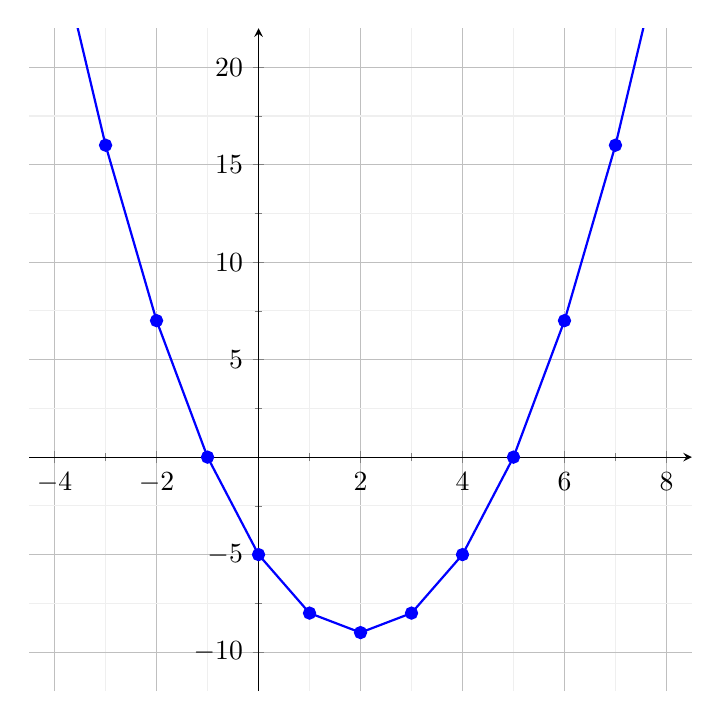
\begin{tikzpicture}
	\begin{axis}[
	xtick distance = 2,
	ytick distance = 5,
	grid = both,	
	minor tick num = 1,
	major grid style = {lightgray},
	minor grid style = {lightgray!25},
	width = 100mm,
	height = 100mm,
	xmin = -4.5, xmax = 8.5,
	ymin = -12, ymax = 22,
	domain = -10:10,
	axis lines = middle,
	]
		
		\addplot[
		samples=21,
		thick,
		blue,
		mark = *,
		] 
		{(x^2)-(4*x)-5};
	\end{axis}
\end{tikzpicture}
\end{subfigure}
\end{figure}

%------------------------------------------------------------------------------
\indent \textbf { 2) $-x^2-6x$ }\\[2mm]
\begin{figure}[h]
	\begin{subfigure}{0.3\textwidth}
		\begin{center}
			\vtablecalc [1]
			{$x$}
			{x=-7,-6,-5,-4,-3,-2,-1,0,1} {$f(x)$}
			{-(x*x)-(6*x)}
		\end{center}
	\end{subfigure}
\begin{subfigure}{0.5\textwidth}
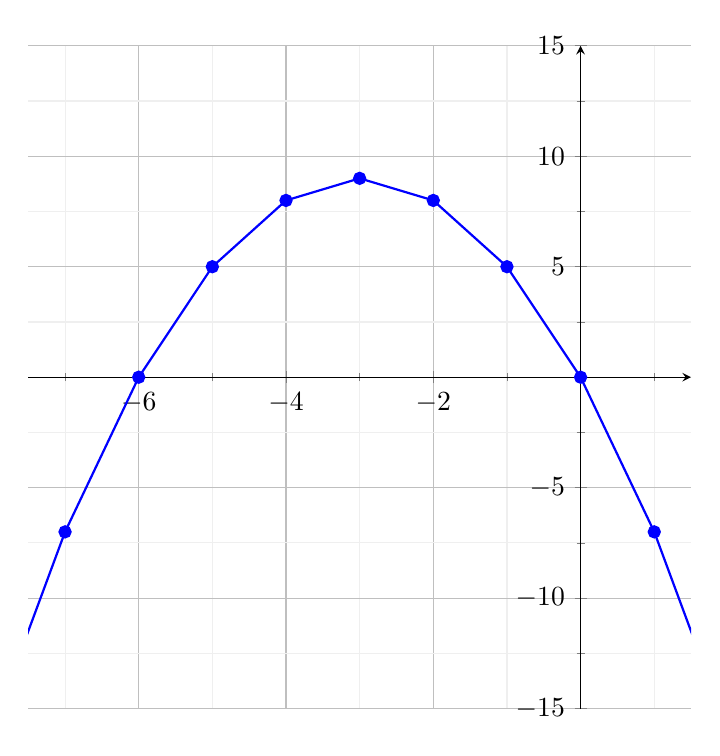
\begin{tikzpicture}
	\begin{axis}[
	xtick distance = 2,
	ytick distance = 5,
	grid = both,	
	minor tick num = 1,
	major grid style = {lightgray},
	minor grid style = {lightgray!25},
	width = 100mm,
	height = 100mm,
	xmin = -7.5, xmax = 1.5,
	ymin = -15, ymax = 15,
	domain = -10:10,
	axis lines = middle,
	]
		
		\addplot[
		samples=21,
		thick,
		blue,
		mark = *,
		] 
		{-(x^2)-(6*x)};
	\end{axis}
\end{tikzpicture}
\end{subfigure}
\end{figure}

%------------------------------------------------------------------------------
\pagebreak \indent \textbf { 3) $x^3-5x^2+2x+8$ }\\[2mm]
\begin{figure}[h]
	\begin{subfigure}{0.2\textwidth}
		%\begin{center}
			\vtablecalc [1]
			{$x$}{x=-9,-8,-7,-6,-5,-4,-3,-2,-1,0,1,2,3,4,5,6,7,8,9}
			{$f(x)$}
			{(x*x*x)-(5*x*x)+(2*x)+8}
		%\end{center}
	\end{subfigure}
\begin{subfigure}{0.7\textwidth}
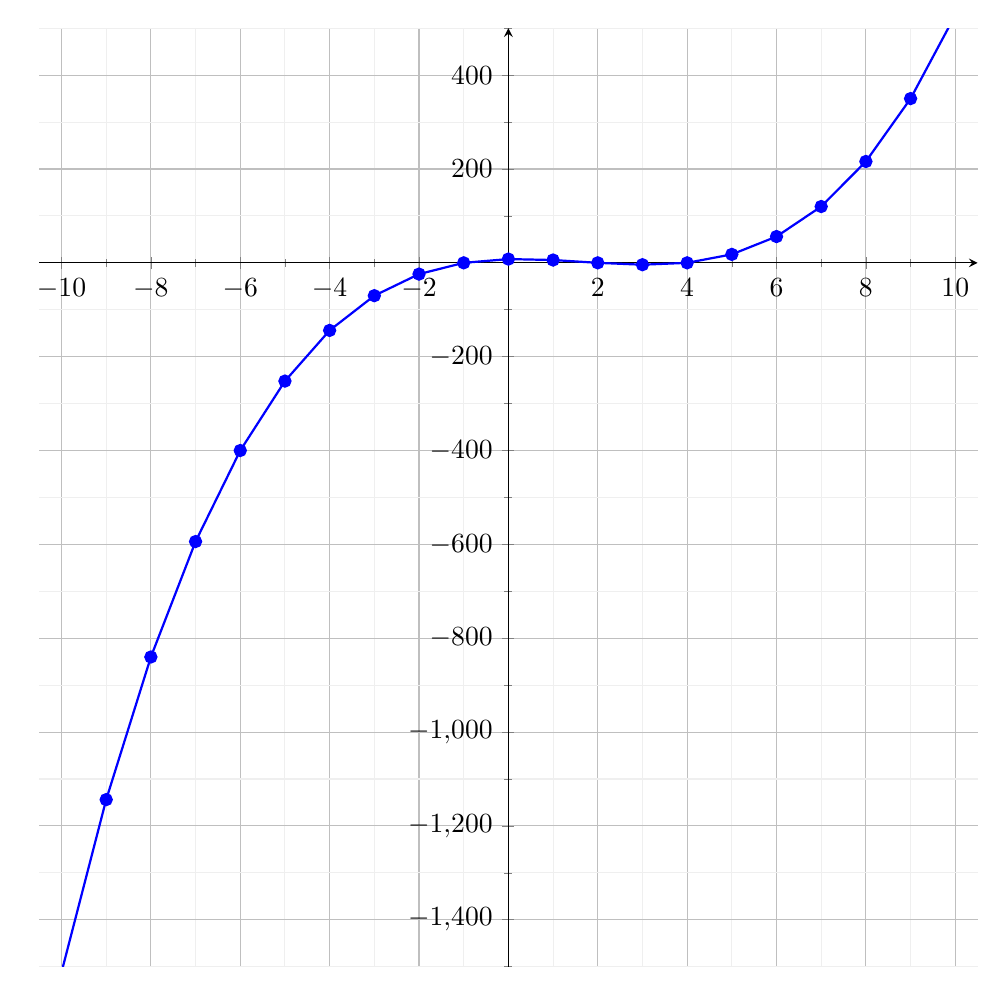
\begin{tikzpicture}
	\begin{axis}[
	xtick distance = 2,
	ytick distance = 200,
	grid = both,	
	minor tick num = 1,
	major grid style = {lightgray},
	minor grid style = {lightgray!25},
	width = 135mm,
	height = 135mm,
	xmin = -10.5, xmax = 10.5,
	ymin = -1500, ymax = 500,
	domain = -10:10,
	axis lines = middle,
	]
		
		\addplot[
		samples=21,
		thick,
		blue,
		mark = *,
		] 
		{(x^3)-(5*x^2)+(2*x)+8};
	\end{axis}
\end{tikzpicture}
\end{subfigure}
\end{figure}

%------------------------------------------------------------------------------
\pagebreak \indent \textbf { 4) $x^3+4x^2-x-4$ }\\[2mm]
\begin{figure}[h]
	\begin{subfigure}{0.2\textwidth}
		%\begin{center}
			\vtablecalc [1]
			{$x$}
			{x=-9,-8,-7,-6,-5,-4,-3,-2,-1,0,1,2,3,4,5,6,7,8,9}
			{$f(x)$}
			{(x*x*x)+(4*x*x)-x-4}
		%\end{center}
	\end{subfigure}
\begin{subfigure}{0.7\textwidth}
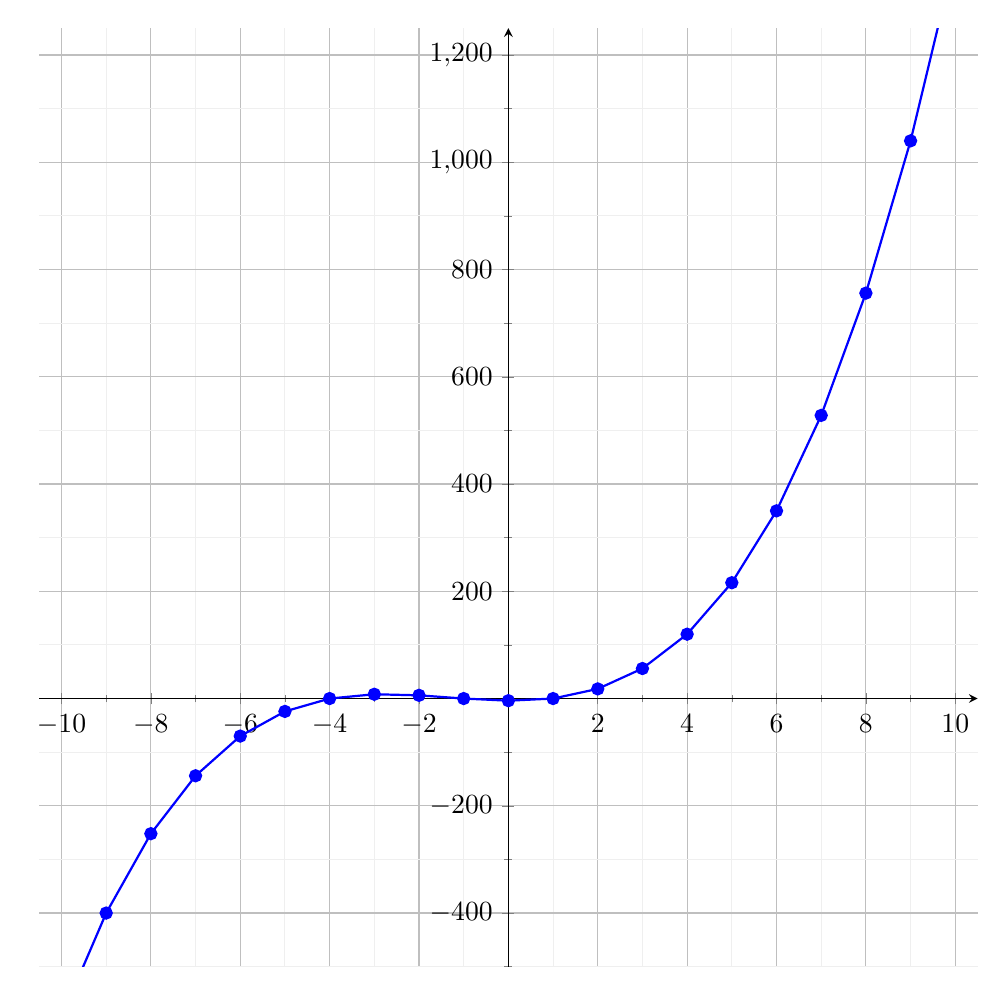
\begin{tikzpicture}
	\begin{axis}[
	xtick distance = 2,
	ytick distance = 200,
	grid = both,	
	minor tick num = 1,
	major grid style = {lightgray},
	minor grid style = {lightgray!25},
	width = 135mm,
	height = 135mm,
	xmin = -10.5, xmax = 10.5,
	ymin = -500, ymax = 1250,
	domain = -10:10,
	axis lines = middle,
	]
		
		\addplot[
		samples=21,
		thick,
		blue,
		mark = *,
		] 
		{(x^3)+(4*x^2)-x-4};
	\end{axis}
\end{tikzpicture}
\end{subfigure}
\end{figure}

%------------------------------------------------------------------------------
\pagebreak \indent \textbf { 5) $f(x) = (x-1) \div (x^2-1)$ }\\[2mm]
Si suponemos que $\dfrac{x-1}{x^2-1}=\dfrac{1}{x+1}$ entonces:
\begin{center}
    \begin{figure}[h]
        \begin{subfigure}{0.4\textwidth}
            %\begin{center}
                \vtablecalc [1]
                {$x$}
                {x=-9,-8,-7,-6,-5,-4,-3,-2,0,2,3,4,5,6,7,8,9} 
                {$f(x)$}
                {1/(x+1)}
            %\end{center}
        \end{subfigure}
        \begin{subfigure}{0.5\textwidth}
			\begin{center}
				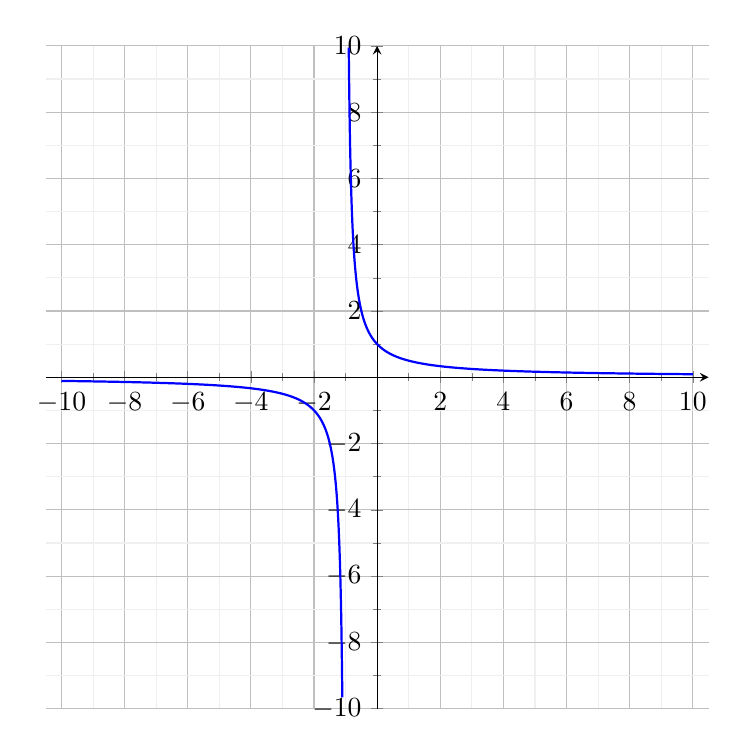
\begin{tikzpicture}
					\begin{axis}[
						xtick distance = 2,
						ytick distance = 2,
						grid = both,	
						minor tick num = 1,
						major grid style = {lightgray},
						minor grid style = {lightgray!25},
						width = 100mm,
						height = 100mm,
						xmin = -10.5, xmax = 10.5,
						ymin = -10, ymax = 10,
						domain = -10:10,
						restrict y to domain=-10:10,
						axis lines = middle,
					]
					\addplot[
						samples=5000,
						thick,
						blue,
						no marks,
					] 
					{1/(x+1)};
					\end{axis}
				\end{tikzpicture}
			\end{center}
        \end{subfigure}
    \end{figure}
\end{center}
%------------------------FUNCIONES TRIGONOMETRICAS-----------------------------
%------------------------------------------------------------------------------
\pagebreak \textbf {Funciones trigonométricas y sus gráficas}\\[2mm]
a) Graficar las siguientes funciones en este rango $-1 < y < 1$ y en este periodo $0 < x < 3\pi$:\\[2mm]
\indent \textbf { 1) $f(x) = 1 + cos(x)$ }\\[2mm]
\begin{center}
\renewcommand{\arraystretch}{2}
\begin{tabular}{|c|c|c|c|c|c|c|c|}
\hline
$x$ &$0$ &$\frac{\pi}{2}$ &$\pi$ &$\frac{3\pi}{2}$ &$2\pi$ &$\frac{5\pi}{2}$ &$3\pi$ \\
\hline
$f(x)$&$2$ &$1$ &$0$ &$1$ &$2$ &$1$ &$0$ \\
\hline
\end{tabular}
\renewcommand{\arraystretch}{1}
\end{center}
\begin{figure}[h]
\begin{center}
\begin{subfigure}{1\textwidth}
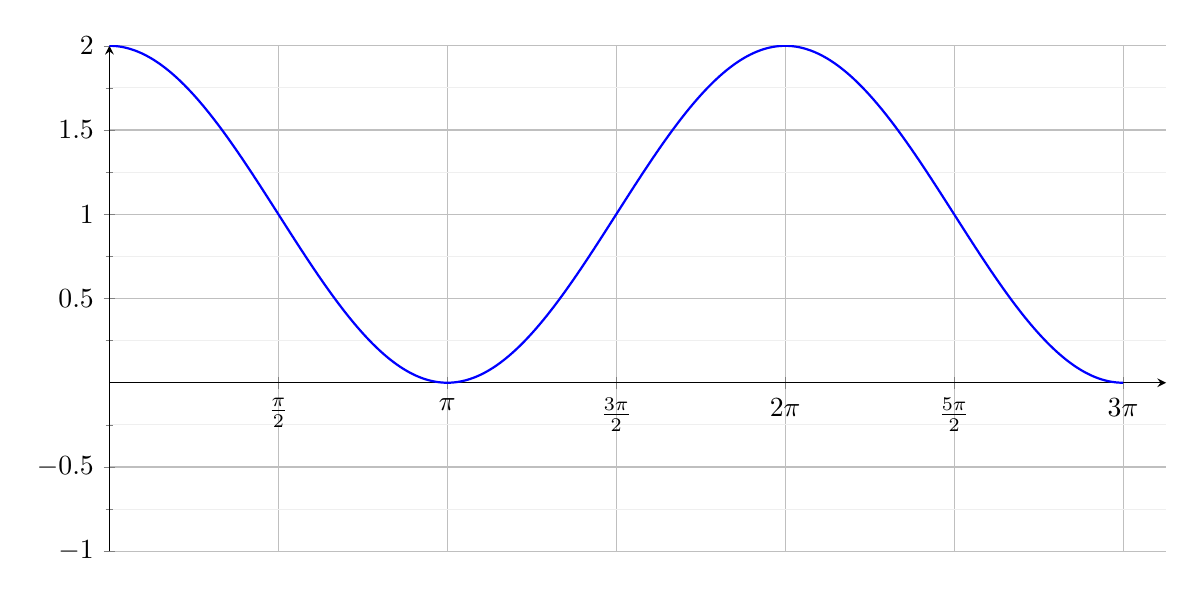
\begin{tikzpicture}
	\begin{axis}[
	xtick = {0,pi/2,pi,pi+pi/2,2*pi,(2*pi)+(pi/2),3*pi},
	xticklabels={$0$,$\frac{\pi}{2}$,$\pi$,$\frac{3\pi}{2}$,$2\pi$,$\frac{5\pi}{2}$,$3\pi$},
	grid = both,	
	minor tick num = 1,
	major grid style = {lightgray},
	minor grid style = {lightgray!25},
	width = 150mm,
	height = 80mm,
	xmin = 0, xmax = 3*pi+.4,
	ymin = -1, ymax = 2,
	domain = 0:3*pi,
	axis lines = middle,
	]
		
		\addplot[
		samples=1000,
		thick,
		blue,
		no marks,
		] 
		{1+cos(deg(x))};
	\end{axis}
\end{tikzpicture}
\end{subfigure}
\end{center}
\end{figure}

%------------------------------------------------------------------------------
\indent \textbf { 2) $f(x) = -sin(x)$ }\\[2mm]
\begin{center}
\renewcommand{\arraystretch}{2}
\begin{tabular}{|c|c|c|c|c|c|c|c|}
\hline
$x$ &$0$ &$\frac{\pi}{2}$ &$\pi$ &$\frac{3\pi}{2}$ &$2\pi$ &$\frac{5\pi}{2}$ &$3\pi$ \\
\hline
$f(x)$&$0$ &$-1$ &$0$ &$1$ &$0$ &$-1$ &$0$ \\
\hline
\end{tabular}
\renewcommand{\arraystretch}{1}
\end{center}
\begin{figure}[h]
\begin{center}
\begin{subfigure}{1\textwidth}
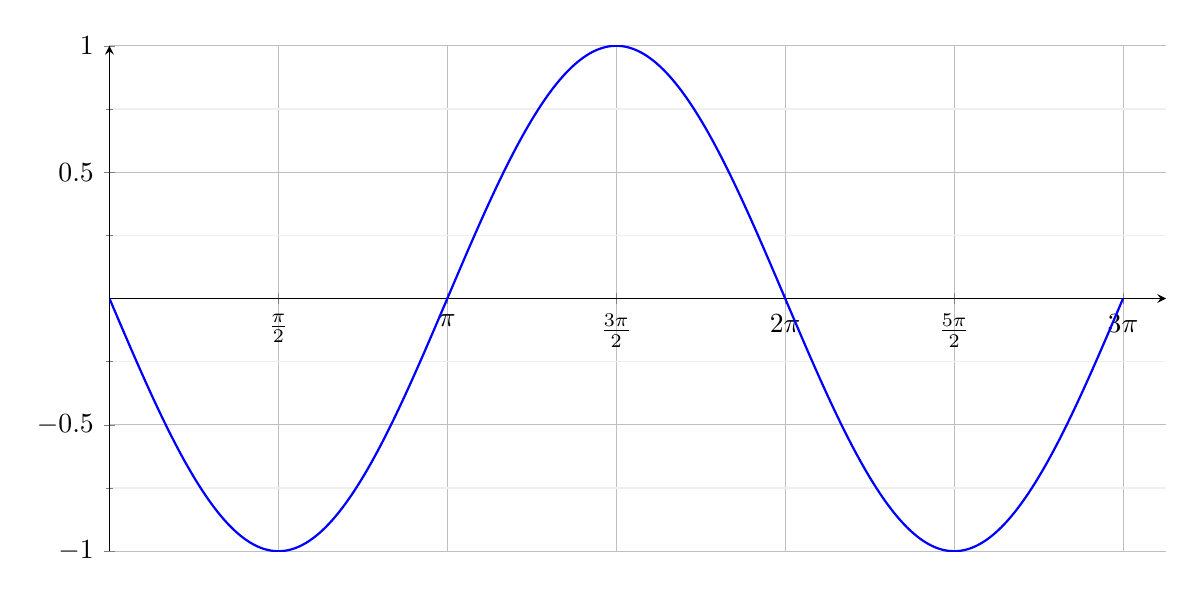
\begin{tikzpicture}
	\begin{axis}[
	xtick = {0,pi/2,pi,pi+pi/2,2*pi,(2*pi)+(pi/2),3*pi},
	xticklabels={$0$,$\frac{\pi}{2}$,$\pi$,$\frac{3\pi}{2}$,$2\pi$,$\frac{5\pi}{2}$,$3\pi$},
	grid = both,	
	minor tick num = 1,
	major grid style = {lightgray},
	minor grid style = {lightgray!25},
	width = 150mm,
	height = 80mm,
	xmin = 0, xmax = 3*pi+.4,
	ymin = -1, ymax = 1,
	domain = 0:3*pi,
	axis lines = middle,
	]
		
		\addplot[
		samples=1000,
		thick,
		blue,
		no marks,
		] 
		{-sin(deg(x))};
	\end{axis}
\end{tikzpicture}
\end{subfigure}
\end{center}
\end{figure}

%------------------------------------------------------------------------------
\pagebreak \indent \textbf { 3) $f(x) = -2 + sin(x)$ }\\[2mm]
\begin{center}
\renewcommand{\arraystretch}{2}
\begin{tabular}{|c|c|c|c|c|c|c|c|}
\hline
$x$ &$0$ &$\frac{\pi}{2}$ &$\pi$ &$\frac{3\pi}{2}$ &$2\pi$ &$\frac{5\pi}{2}$ &$3\pi$ \\
\hline
$f(x)$&$-2$ &$-1$ &$-2$ &$-3$ &$-2$ &$-1$ &$-2$ \\
\hline
\end{tabular}
\renewcommand{\arraystretch}{1}
\end{center}
\begin{figure}[h]
\begin{center}
\begin{subfigure}{1\textwidth}
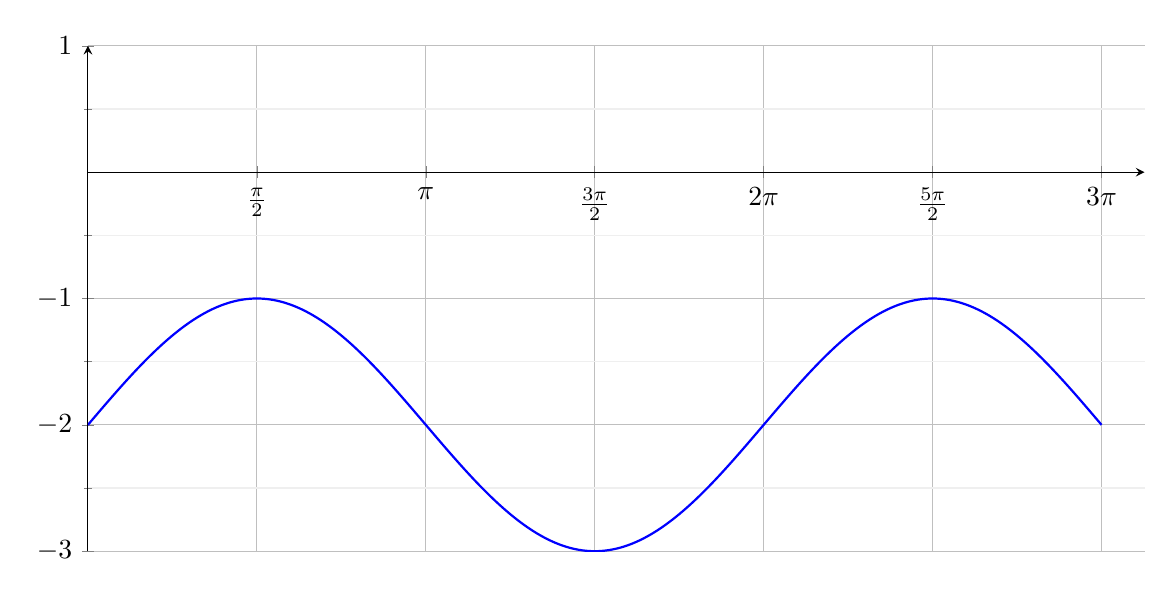
\begin{tikzpicture}
	\begin{axis}[
	xtick = {0,pi/2,pi,pi+pi/2,2*pi,(2*pi)+(pi/2),3*pi},
	xticklabels={$0$,$\frac{\pi}{2}$,$\pi$,$\frac{3\pi}{2}$,$2\pi$,$\frac{5\pi}{2}$,$3\pi$},
	grid = both,	
	minor tick num = 1,
	major grid style = {lightgray},
	minor grid style = {lightgray!25},
	width = 150mm,
	height = 80mm,
	xmin = 0, xmax = 3*pi+.4,
	ymin = -3, ymax = 1,
	domain = 0:3*pi,
	axis lines = middle,
	]
		
		\addplot[
		samples=1000,
		thick,
		blue,
		no marks,
		] 
		{-2 + (sin(deg(x)))};
	\end{axis}
\end{tikzpicture}
\end{subfigure}
\end{center}
\end{figure}

%------------------------------------------------------------------------------
\indent \textbf { 4) $f(x) = 3 cos(x)$ }\\[2mm]
\begin{center}
\renewcommand{\arraystretch}{2}
\begin{tabular}{|c|c|c|c|c|c|c|c|}
\hline
$x$ &$0$ &$\frac{\pi}{2}$ &$\pi$ &$\frac{3\pi}{2}$ &$2\pi$ &$\frac{5\pi}{2}$ &$3\pi$ \\
\hline
$f(x)$&$3$ &$0$ &$-3$ &$0$ &$3$ &$0$ &$-3$ \\
\hline
\end{tabular}
\renewcommand{\arraystretch}{1}
\end{center}
\begin{figure}[h]
\begin{center}
\begin{subfigure}{1\textwidth}
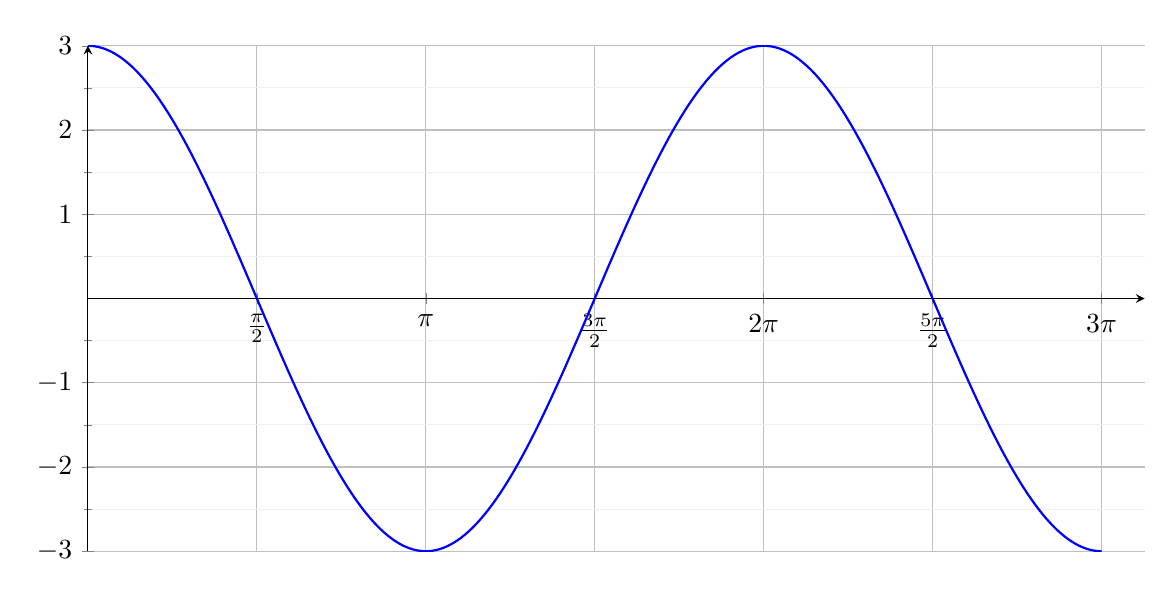
\begin{tikzpicture}
	\begin{axis}[
	xtick = {0,pi/2,pi,pi+pi/2,2*pi,(2*pi)+(pi/2),3*pi},
	xticklabels={$0$,$\frac{\pi}{2}$,$\pi$,$\frac{3\pi}{2}$,$2\pi$,$\frac{5\pi}{2}$,$3\pi$},
	grid = both,	
	minor tick num = 1,
	major grid style = {lightgray},
	minor grid style = {lightgray!25},
	width = 150mm,
	height = 80mm,
	xmin = 0, xmax = 3*pi+.4,
	ymin = -3, ymax = 3,
	domain = 0:3*pi,
	axis lines = middle,
	]
		
		\addplot[
		samples=1000,
		thick,
		blue,
		no marks,
		] 
		{3 * (cos(deg(x)))};
	\end{axis}
\end{tikzpicture}
\end{subfigure}
\end{center}
\end{figure}

%---------------------------FUNCIONES LOGARITMICAS-----------------------------
%------------------------------------------------------------------------------
\pagebreak \textbf {Funciones logarítmicas y sus gráficas}\\[2mm]
a) Graficar las siguientes funciones logarítmicas:\\[2mm]
\indent \textbf { 1) $f(x) = log_{10}(x)$ }\\[2mm]
\begin{center}
\begin{tabular}{|c|c|c|c|c|c|c|c|c|c|c|c|}
\hline
$x$&$0.01$&$0.1$&$0.25$&$0.5$&$0.75$&$1$&$1.5$&$2$&$2.5$&$3$&$5$ \\
\hline
$f(x)$&$-2$&$-1$&$-0.6$&$-0.3$&$-0.125$&$0$&$0.176$&$0.301$&$0.3979$&$0.4771$&$0.6989$ \\
\hline
\end{tabular}
\end{center}
\begin{figure}[h]
\begin{subfigure}{1\textwidth}
\begin{center}
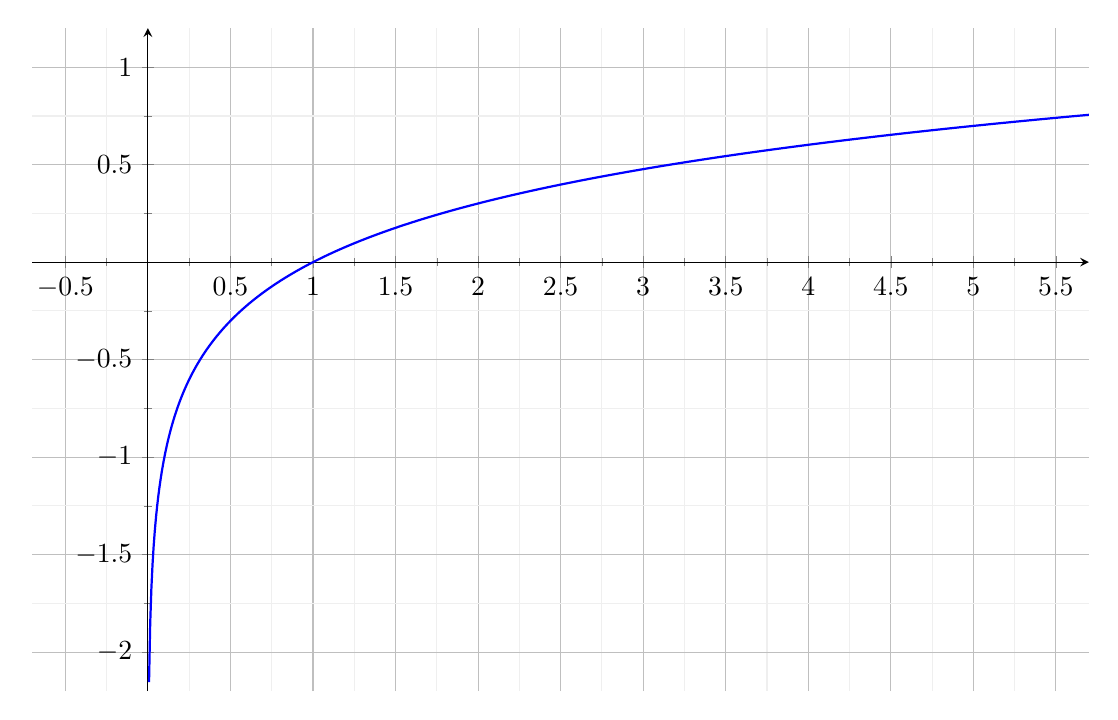
\begin{tikzpicture}
	\begin{axis}[
	xtick distance = .5,
	ytick distance = .5,
	grid = both,	
	minor tick num = 1,
	major grid style = {lightgray},
	minor grid style = {lightgray!25},
	width = 150mm,
	height = 100mm,
	xmin = -0.7, xmax = 5.7,
	ymin = -2.2, ymax = 1.2,
	domain = 0:7,
	axis lines = middle,
	]
		
		\addplot[
		samples=1000,
		thick,
		blue,
		no marks,
		] 
		{log10(x)};
	\end{axis}
\end{tikzpicture}
\end{center}
\end{subfigure}
\end{figure}

%------------------------------------------------------------------------------
\indent \textbf { 2) $f(x) = ln (x)$ }\\[2mm]
\begin{center}
\begin{tabular}{|c|c|c|c|c|c|c|c|c|c|c|c|}
\hline
$x$&$0.01$&$0.1$&$0.25$&$0.5$&$0.75$&$1$&$1.5$&$2$&$2.5$&$3$&$5$ \\
\hline
$f(x)$&$-4.6$&$-2.3$&$-1.3862$&$-0.6931$&$-0.2876$&$0$&$0.4054$&$0.69$&$0.91$&$1.09$&$1.61$ \\
\hline
\end{tabular}
\end{center}
\begin{figure}[h]
\begin{subfigure}{1\textwidth}
\begin{center}
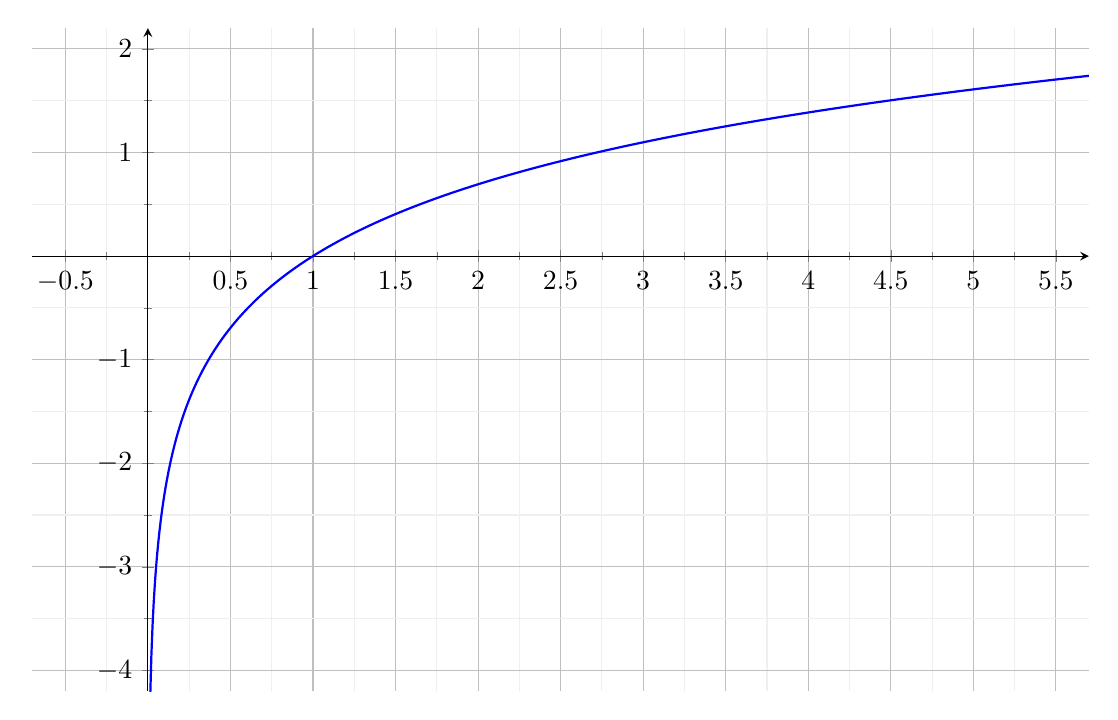
\begin{tikzpicture}
	\begin{axis}[
	xtick distance = .5,
	ytick distance = 1,
	grid = both,	
	minor tick num = 1,
	major grid style = {lightgray},
	minor grid style = {lightgray!25},
	width = 150mm,
	height = 100mm,
	xmin = -0.7, xmax = 5.7,
	ymin = -4.2, ymax = 2.2,
	domain = 0:7,
	axis lines = middle,
	]
		
		\addplot[
		samples=1000,
		thick,
		blue,
		no marks,
		] 
		{ln(x)};
	\end{axis}
\end{tikzpicture}
\end{center}
\end{subfigure}
\end{figure}

%------------------------------------------------------------------------------
\pagebreak \indent \textbf { 3) $f(x) = e^x$ }\\[2mm]
\begin{center}
\begin{tabular}{|c|c|c|c|c|c|c|c|c|c|c|c|}
\hline
$x$&$-3.5$&$-1.5$&$-1$&$-0.5$&$0$&$0.5$&$1$&$1.5$&$2$&$2.5$&$3$ \\
\hline
$f(x)$&$0.03$&$0.22$&$0.3678$&$0.6065$&$1$&$1.6487$&$2.71$&$4.48$&$7.39$&$12.18$&$20.08$ \\
\hline
\end{tabular}
\end{center}
\begin{figure}[h]
\begin{subfigure}{1\textwidth}
\begin{center}
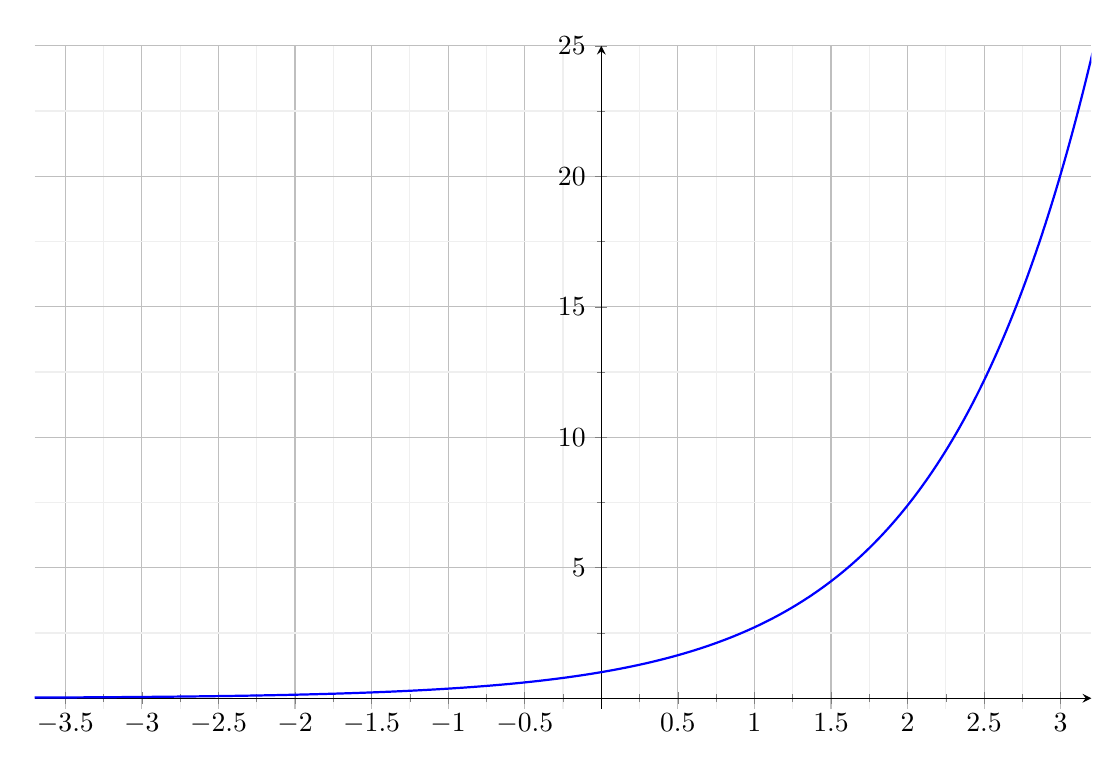
\begin{tikzpicture}
	\begin{axis}[
	xtick distance = .5,
	ytick distance = 5,
	grid = both,	
	minor tick num = 1,
	major grid style = {lightgray},
	minor grid style = {lightgray!25},
	width = 150mm,
	height = 100mm,
	xmin = -3.7, xmax = 3.2,
	ymin = -0.4, ymax = 25,
	domain = -4:7,
	axis lines = middle,
	]
		
		\addplot[
		samples=1000,
		thick,
		blue,
		no marks,
		] 
		{e^(x)};
	\end{axis}
\end{tikzpicture}
\end{center}
\end{subfigure}
\end{figure}

%------------------------ANGULOS, GRADOS Y RADIANES----------------------------
%------------------------------------------------------------------------------
\pagebreak \textbf {Ángulos, grados y radianes}\\[2mm]
a) Encontrar los valores siguientes:\\[2mm]
\indent \textbf { 1)} Valor de $\alpha$ y $\beta$ \\[2mm]
\begin{center}
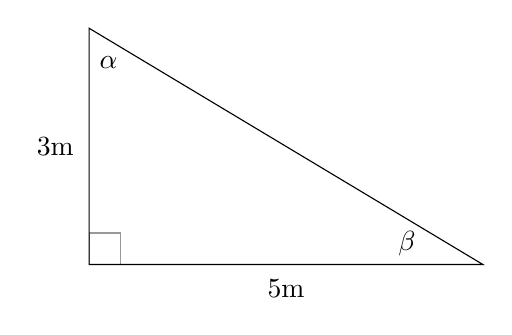
\begin{tikzpicture}[]
\coordinate (O) at (0,0);
\coordinate (A) at (5,0);
\coordinate (B) at (0,3);
\draw (O)--(A)--(B)--cycle;

\tkzLabelSegment[below=2pt](O,A){5m}
\tkzLabelSegment[left=2pt](O,B){3m}
\tkzLabelSegment[above right=2pt](A,B){}

\tkzMarkRightAngle[size=0.4,opacity=.4](A,O,B)% square angle here
\tkzLabelAngle[pos = 0.35](A,O,B){}


\tkzLabelAngle[pos = 1](B,A,O){$\beta$}

\tkzLabelAngle[pos = 0.5](O,B,A){$\alpha$}


\end{tikzpicture}
\end{center}
Para obtener los angulos $\alpha$ y $\beta$, debemos conocer que: 

$$Sin\theta=\frac{cateto\:opuesto}{hipotenusa} \qquad Cos\theta=\frac{cateto\:adyacente}{hipotenusa} \qquad Tan\theta=\frac{cateto\:opuesto}{cateto\:adyacente}$$

Para el angulo $\alpha$ nuestra formula quedaría:

$$Tan\alpha=\frac{5m}{3m}$$

Para despejar el angulo, debemos eliminar la tangente con su inverso en ambos lados:

$$Tan^{-1}\left(Tan\alpha\right)=Tan^{-1}\left(\frac{5m}{3m}\right)$$
$$\alpha=Tan^{-1}\left(\frac{5m}{3m}\right)$$
$$\alpha=59.0362$$
$$\alpha=59^{\circ}2'10.4765''$$

Para el angulo $\beta$ nuestra formula quedaría:

$$Tan\beta=\frac{3m}{5m}$$

Eliminamos la tangente con su inverso en ambos lados:

$$Tan^{-1}\left(Tan\beta\right)=Tan^{-1}\left(\frac{3m}{5m}\right)$$
$$\beta=Tan^{-1}\left(\frac{3m}{5m}\right)$$
$$\beta=30.9637$$
$$\beta=30^{\circ}57'49.5235''$$

%------------------------------------------------------------------------------
\pagebreak \indent \textbf { 2)} Calcular $sin(\alpha)$, $cos(\beta)$, $tan(\alpha)$, $cot(\beta)$, $sec(\alpha)$ y $csc(\beta)$ \\[2mm]
Si $h=\sqrt{a^2+b^2}$, entonces $h=\sqrt{34}$, entonces:
\begin{center}
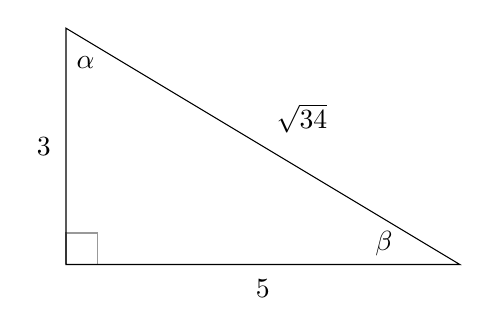
\begin{tikzpicture}[]
\coordinate (O) at (0,0);
\coordinate (A) at (5,0);
\coordinate (B) at (0,3);
\draw (O)--(A)--(B)--cycle;

\tkzLabelSegment[below=2pt](O,A){5}
\tkzLabelSegment[left=2pt](O,B){3}
\tkzLabelSegment[above right=2pt](A,B){$\sqrt{34}$}

\tkzMarkRightAngle[size=0.4,opacity=.4](A,O,B)% square angle here
\tkzLabelAngle[pos = 0.35](A,O,B){}


\tkzLabelAngle[pos = 1](B,A,O){$\beta$}

\tkzLabelAngle[pos = 0.5](O,B,A){$\alpha$}


\end{tikzpicture}
\end{center}
Ademas sabemos que:

$$Sin\theta=\frac{cateto\:opuesto}{hipotenusa} \qquad Cos\theta=\frac{cateto\:adyacente}{hipotenusa} \qquad Tan\theta=\frac{cateto\:opuesto}{cateto\:adyacente}$$
$$Cot\theta=\frac{cateto\:adyacente}{cateto\:opuesto} \qquad Sec\theta=\frac{hipotenusa}{cateto\:adyacente} \qquad Csc\theta=\frac{hipotenusa}{cateto\:opuesto}$$

Entonces: \\[2mm]
$$Sin\alpha=\dfrac{5}{\sqrt{34}}=0.8575$$ \\[2mm]
$$Cos\beta=\dfrac{5}{\sqrt{34}}=0.8575$$ \\[2mm]
$$Tan\alpha=\dfrac{5}{3}=1.6$$ \\[2mm]
$$Cot\beta=\dfrac{5}{3}=1.6$$ \\[2mm]
$$Sec\alpha=\dfrac{\sqrt{34}}{3}=1.9436$$ \\[2mm]
$$Csc\beta=\dfrac{\sqrt{34}}{3}=1.9436$$ \\[2mm]

%------------------------------------------------------------------------------
\pagebreak \indent \textbf { 3)} Convertir a radianes los valores de $\alpha$ y de $\beta$ \\[2mm]
Para convertir grados a radianes necesitamos conocer que: $\pi_{rad}=180^{\circ}$ \\[2mm]
Si $\alpha=59.0362$, utilizamos la siguiente conversión:

$$\alpha=59.0362\left(\frac{\pi}{180}\right)$$
$$\alpha=1.030376$$

Y para $\beta=30.9637$:

$$\beta=30.9637\left(\frac{\pi}{180}\right)$$
$$\beta=0.540419$$


\indent \textbf { 4)} Convertir grados centecimales los valores de $\alpha$ y de $\beta$ \\[2mm]
Para convertir radianes a grados centecimales necesitamos conocer que: $\dfrac{centesimal}{200}=\dfrac{radian}{\pi}$ \\[2mm]
Entonces: 
$$centesimal=\dfrac{(200)(radian)}{\pi}$$

Si los resultados en radianes son $\alpha=1.030376$:

$$\alpha=\dfrac{(200)(1.030376)}{\pi}$$
$$\alpha=65.5957$$

Y para $\beta=0.540419$:

$$\beta=\dfrac{(200)(0.540419)}{\pi}$$
$$\beta=34.4041$$

%---------------------------------------B--------------------------------------
%------------------------------------------------------------------------------
\pagebreak b) Encontrar los valores siguientes:\\[2mm]
\indent \textbf { 1)} Valor de $\alpha$ y $\beta$ \\[2mm]
\begin{center}
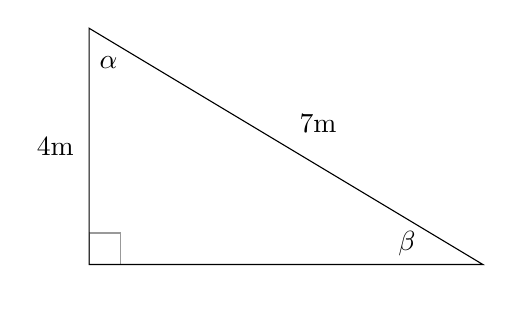
\begin{tikzpicture}[]
\coordinate (O) at (0,0);
\coordinate (A) at (5,0);
\coordinate (B) at (0,3);
\draw (O)--(A)--(B)--cycle;

\tkzLabelSegment[below=2pt](O,A){}
\tkzLabelSegment[left=2pt](O,B){4m}
\tkzLabelSegment[above right=2pt](A,B){7m}

\tkzMarkRightAngle[size=0.4,opacity=.4](A,O,B)% square angle here
\tkzLabelAngle[pos = 0.35](A,O,B){}


\tkzLabelAngle[pos = 1](B,A,O){$\beta$}

\tkzLabelAngle[pos = 0.5](O,B,A){$\alpha$}


\end{tikzpicture}
\end{center}
Para obtener los angulos $\alpha$ y $\beta$, debemos conocer que: 

$$Sin\theta=\frac{cateto\:opuesto}{hipotenusa} \qquad Cos\theta=\frac{cateto\:adyacente}{hipotenusa} \qquad Tan\theta=\frac{cateto\:opuesto}{cateto\:adyacente}$$

Para el angulo $\alpha$ nuestra formula quedaría:

$$Cos\alpha=\frac{4m}{7m}$$

Para despejar el angulo, debemos eliminar el coseno con su inverso en ambos lados:

$$Cos^{-1}\left(Cos\alpha\right)=Cos^{-1}\left(\frac{4m}{7m}\right)$$
$$\alpha=Cos^{-1}\left(\frac{4m}{7m}\right)$$
$$\alpha=55.1501$$
$$\alpha=55^{\circ}9'0.343515''$$

Para el angulo $\beta$ nuestra formula quedaría:

$$Tan\beta=\frac{4m}{7m}$$

Eliminamos la tangente con su inverso en ambos lados:

$$Tan^{-1}\left(Tan\beta\right)=Tan^{-1}\left(\frac{4m}{7m}\right)$$
$$\beta=Tan^{-1}\left(\frac{4m}{7m}\right)$$
$$\beta=29.7449$$
$$\beta=29^{\circ}44'41.5727''$$

%------------------------------------------------------------------------------
\pagebreak \indent \textbf { 2)} Calcular $sin(\alpha)$, $cos(\beta)$, $tan(\alpha)$, $cot(\beta)$, $sec(\alpha)$ y $csc(\beta)$ \\[2mm]
Si $b=\sqrt{h^2+a^2}$, entonces $b=\sqrt{65}$, entonces:
\begin{center}
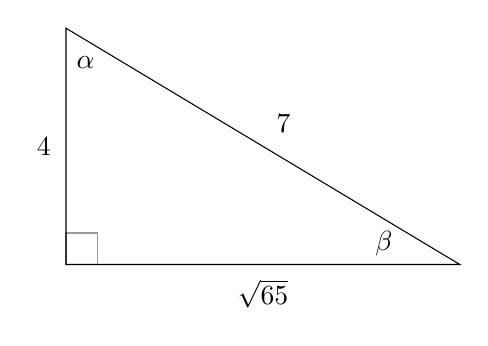
\begin{tikzpicture}[]
\coordinate (O) at (0,0);
\coordinate (A) at (5,0);
\coordinate (B) at (0,3);
\draw (O)--(A)--(B)--cycle;

\tkzLabelSegment[below=2pt](O,A){$\sqrt{65}$}
\tkzLabelSegment[left=2pt](O,B){4}
\tkzLabelSegment[above right=2pt](A,B){7}

\tkzMarkRightAngle[size=0.4,opacity=.4](A,O,B)% square angle here
\tkzLabelAngle[pos = 0.35](A,O,B){}


\tkzLabelAngle[pos = 1](B,A,O){$\beta$}

\tkzLabelAngle[pos = 0.5](O,B,A){$\alpha$}


\end{tikzpicture}
\end{center}
Ademas sabemos que:

$$Sin\theta=\frac{cateto\:opuesto}{hipotenusa} \qquad Cos\theta=\frac{cateto\:adyacente}{hipotenusa} \qquad Tan\theta=\frac{cateto\:opuesto}{cateto\:adyacente}$$
$$Cot\theta=\frac{cateto\:adyacente}{cateto\:opuesto} \qquad Sec\theta=\frac{hipotenusa}{cateto\:adyacente} \qquad Csc\theta=\frac{hipotenusa}{cateto\:opuesto}$$

Entonces: \\[2mm]
$$Sin\alpha=\dfrac{\sqrt{65}}{7}=1.1517$$ \\[2mm]
$$Cos\beta=\dfrac{\sqrt{65}}{7}=1.1517$$ \\[2mm]
$$Tan\alpha=\dfrac{\sqrt{65}}{4}=2.0155$$ \\[2mm]
$$Cot\beta=\dfrac{\sqrt{65}}{4}=2.0155$$ \\[2mm]
$$Sec\alpha=\dfrac{7}{4}=1.75$$ \\[2mm]
$$Csc\beta=\dfrac{7}{4}=1.75$$ \\[2mm]

%------------------------------------------------------------------------------
\pagebreak \indent \textbf { 3)} Convertir a radianes los valores de $\alpha$ y de $\beta$ \\[2mm]
Para convertir grados a radianes necesitamos conocer que: $\pi_{rad}=180^{\circ}$ \\[2mm]
Si $\alpha=55.1501$, utilizamos la siguiente conversión:

$$\alpha=55.1501\left(\frac{\pi}{180}\right)$$
$$\alpha=0.962550$$

Y para $\beta=29.7449$:

$$\beta=29.7449\left(\frac{\pi}{180}\right)$$
$$\beta=0.519146$$


\indent \textbf { 4)} Convertir grados centecimales los valores de $\alpha$ y de $\beta$ \\[2mm]
Para convertir radianes a grados centecimales necesitamos conocer que: $\dfrac{centesimal}{200}=\dfrac{radian}{\pi}$ \\[2mm]
Entonces: 
$$centesimal=\dfrac{(200)(radian)}{\pi}$$

Si los resultados en radianes son $\alpha=0.962550$:

$$\alpha=\dfrac{(200)(0.962550)}{\pi}$$
$$\alpha=61.2778$$

Y para $\beta=0.519146$:

$$\beta=\dfrac{(200)(0.519146)}{\pi}$$
$$\beta=33.0498$$

%-----------------------------LIMITES Y CONTINUIDAD----------------------------
%------------------------------------------------------------------------------
\pagebreak \textbf {Límites y continuidad}\\[2mm]
a) Elaborar un documento de una hoja por lo menos donde se exponga qué es un límite de una función y cinco (5) ejemplos en una hoja adicional.
\begin{wrapfigure}{1}{0.35\textwidth}
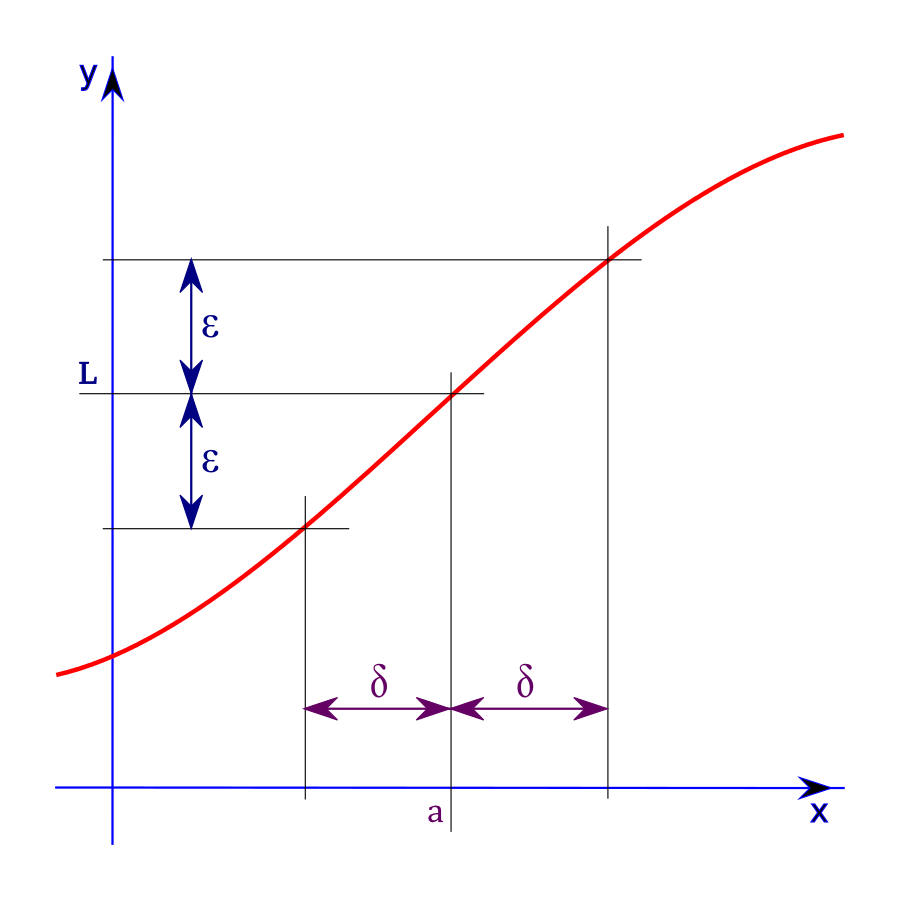
\includegraphics[width=0.35\textwidth]{lim}
\caption*{\textbf{Figura 1.} Visualización de los parámetros de un límite}
\label{figu:mesh1}
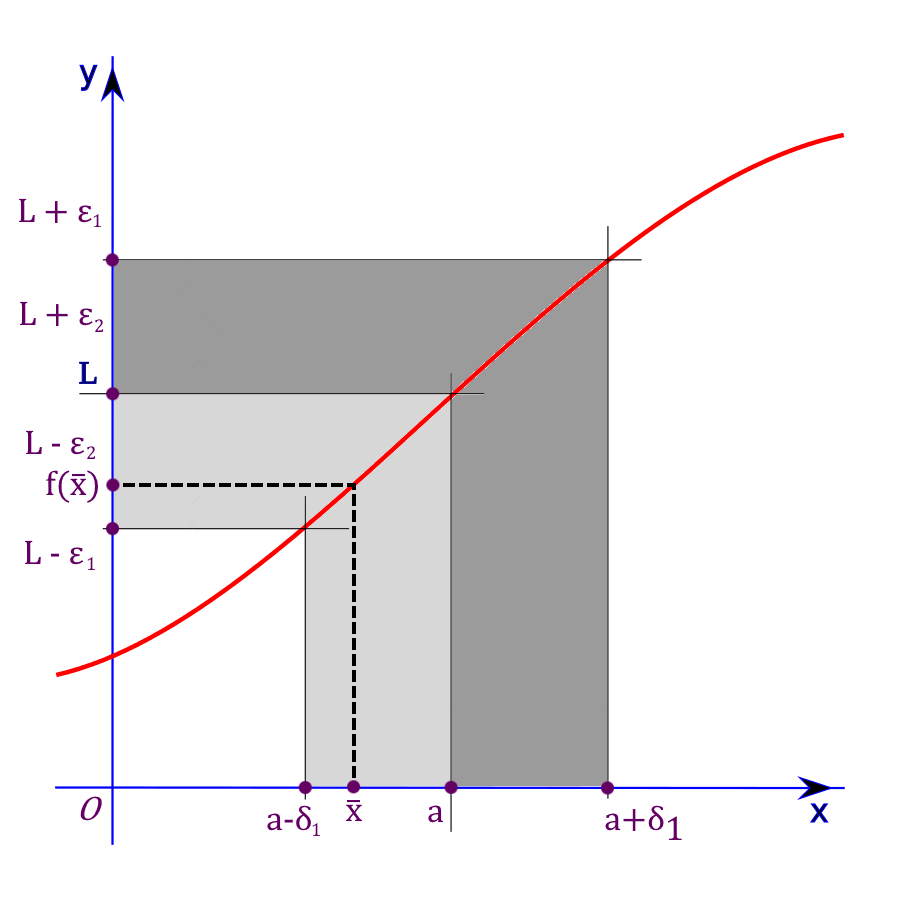
\includegraphics[width=0.35\textwidth]{lim2}
\caption*{\textbf{Figura 2.}}
\label{figu:mesh2}
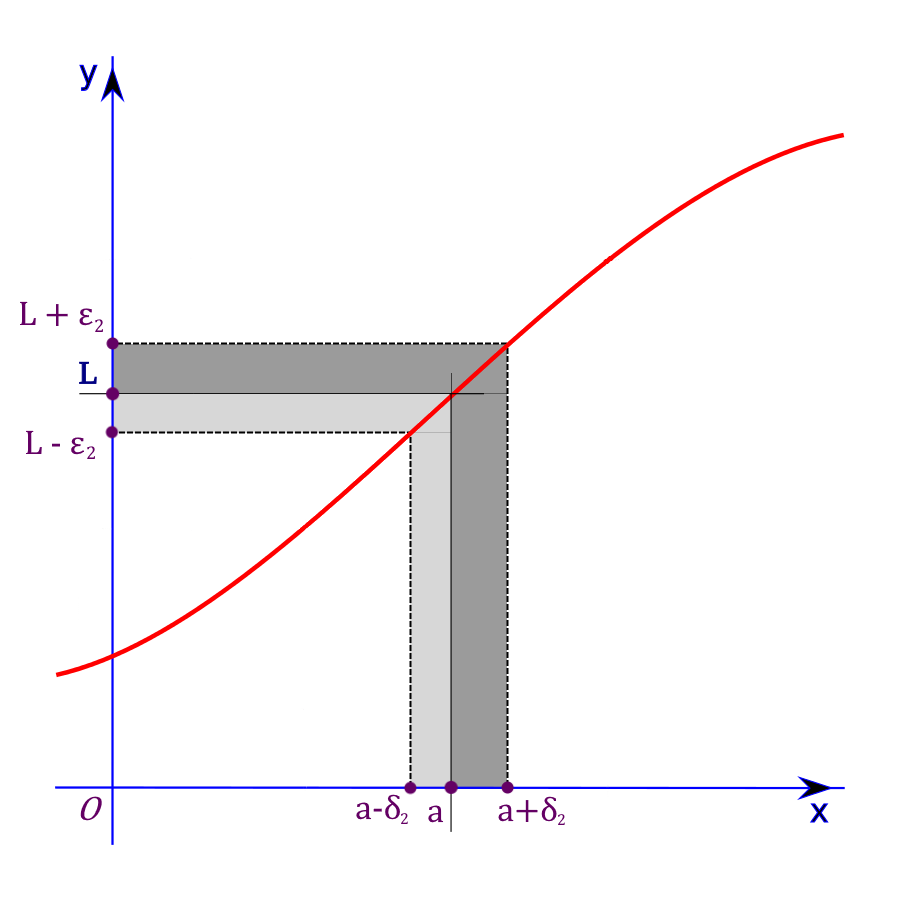
\includegraphics[width=0.35\textwidth]{lim3}
\caption*{\textbf{Figura 3.}}
\label{figu:mesh3}
\end{wrapfigure}

\hspace*{10mm}La definición formal de límite de una función dice que: Sea $f$ una función definida en cada número de algún intervalo abierto que contiene a $a$, excepto posiblemente en el número $a$ mismo. El límite de $f(x)$ conforme $x$ se aproxima a $a$ es $L$, lo que se escribe como:

$$\lim_{x \to a}f(x)=L$$

\hspace*{10mm}En otras palabras, esta definición establece que los valores de función $f(x)$ se aproximan al límite $L$ conforme $x$ lo hace al número $a$ si el valor absoluto de la diferencia entre $f(x)$ y $L$ puede hacerse tan pequeña como se desee tomando $x$ suficientemente cerca de $a$ pero no igual a $a$.

\hspace*{10mm}Observe que no se menciona nada acerca del valor de la función cuando $x=a$. La función $f$ no necesita estar definida en $a$, para que el $\lim_{x \to a}f(x)$ exista. Más aún, si $f$ está definida en $a$, $\lim_{x \to a}f(x)$ puede existir sin que tenga el mismo valor que $f(a)$.

\hspace*{10mm}Una interpretación geométrica de la definición de límite de una función $f$ se muestra en la \textbf{Figura 1}, la cual presenta una porción de la gráfica de $f$ cerca del punto donde $x = a$. Como $f$ no está necesariamente definida en $a$, no existe un punto en la gráfica de $f$ con abscisa $a$. Observe que si $x$, en el eje horizontal, está entre $a - \delta_1$ y $a + \delta_1$, entonces $f(x)$, en el eje vertical, estará entre $L - \epsilon_1$ y $L + \epsilon_1$. Así, $$\text{si }0 < |x-a| < \delta_1\text{   entonces }|f(x) - L < \epsilon_1$$

La \textbf{Figura 2} muestra cómo un valor pequeño de $\epsilon$ puede requerir una elección diferente para $\delta$. En la figura se aprecia que $\epsilon_2 < \epsilon_1$, y que el valor $\delta_1$ es demasiado grande; esto es, existen valores de x para los cuales $0 < |x-a| < \delta_1$, pero $|f(\overline{x} - L|$ no es menor que $\epsilon_2$. Por ejemplo, $0 < |x-a| < \delta_2$. Por esta razón debe elegirse un valor $\delta_2$ más pequeño, como se muestra en la \textbf{Figura 3}, tal que $$\text{si }0 < |x-a| < \delta_2\text{ entonces }|f(x) - L| < \epsilon_2$$

Sin embargo, para cualquier elección de $\epsilon > 0$, no importa que tan pequeño sea, existe $\delta > 0$ tal que la proposición (1) se cumple. Por tanto, $\lim_{x \to a}f(x)=L$. 

\pagebreak \textbf{Ejemplos.}

1) $\lim_{x\to5} (3x+1)$\\[2mm]
Sustituimos 5 en la función:
$$\lim_{x\to5} (3x+1) = (3(5)+1)$$
$$=(15)+1 = 16$$

2) $\lim_{x\to5} (2x^2-5x+3)$\\[2mm]
$$=2(5)^2-5(5)+3$$
$$=2(25)-25+3$$
$$=50-25+3$$
$$=28$$

3) $\lim_{x\to-4} (x^3-2x^2+x+8)$\\[2mm]
$$=(-4)^3-2(-4)^2+(-4)+8$$
$$=(-64)-2(16)-4+8$$
$$=-64-32-4+8$$
$$=-92$$

4) $\lim_{x\to-2} (3x^3-10x^2-4)$\\[2mm]
$$=3(-2)^3-10(-2)^2-4$$
$$=3(-8)-10(4)-4$$
$$=-24-40-4$$
$$=-68$$

5) $\lim_{x\to4} \left(\dfrac{8x^2+2}{x-2}\right)$\\[2mm]
$$=\left(\dfrac{8(4)^2+2}{(4)-2}\right)$$
$$=\left(\dfrac{8(16)+2}{2}\right)$$
$$=\left(\dfrac{130}{2}\right)$$
$$=65$$

%-----------------------------LIMITES Y CONTINUIDAD----------------------------
%-------------------------------------LEYES------------------------------------
\pagebreak \textbf{Leyes de Límites.}\\[2mm]
Suponga que \textit{c} es una constante y que existen los límites
$$\lim_{x \to a}f(x)\qquad \text{y} \qquad\lim_{x \to a}g(x)$$
Entonces\\[2mm]
\textbf{1. }\textit{El límite de la suma de límites es la suma de los límites.}
$$\lim_{x \to a}[f(x) + g(x)] = \lim_{x \to a}f(x) + \lim_{x \to a}g(x)$$
\textbf{2. }\textit{El límite de una diferencia es la diferencia de los límites.}
$$\lim_{x \to a}[f(x) - g(x)] = \lim_{x \to a}f(x) - \lim_{x \to a}g(x)$$
\textbf{3. }\textit{El límite de una constante por una función es la constante por el límite de la función.}
$$\lim_{x \to a}[cf(x)] = c\lim_{x \to a}f(x)$$
\textbf{4. }\textit{El límite de un producto es el producto de los límites.}
$$\lim_{x \to a}[f(x)g(x)] = \lim_{x \to a}f(x) \cdot \lim_{x \to a}g(x)$$
\textbf{5. }\textit{El límite de un cociente es el cociente de los límites, siempre que el límite del denominador no sea 0.}
$$\lim_{x \to a}\frac{f(x)}{g(x)}=\frac{\lim_{x \to a}f(x)}{\lim_{x \to a}g(x)} \quad \text{si }\lim_{x \to a}g(x) \neq 0$$
\textbf{6. }\textit{El límite de una potencia es la potencia del limite.}
$$\lim_{x \to a}[f(x)]^n=[\lim_{x \to a}f(x)]^n$$
\textbf{7. }\textit{El límite de una raíz es la raíz del limite.}
$$\lim_{x \to a}\sqrt[n]{f(x)}=\sqrt[n]{\lim_{x \to a}f(x)} \quad \text{donde }n\text{ es un entero positivo}$$
$$[\text{Si }n \text{ es par, suponemos que }\lim_{x \to a}f(x)>0.]$$\\[2mm]

\textbf{Limites especiales}\\[2mm]
\textbf{1. }$\lim_{x \to a}c=c$\\[2mm]
\textbf{2. }$\lim_{x \to a}x=a$\\[2mm]
\textbf{3. }$\lim_{x \to a}x^n=a^n \qquad$donde $n$ es un entero positivo\\[2mm]
\textbf{4. }$\lim_{x \to a}\sqrt[n]{x}=\sqrt[n]{a} \qquad$donde $n$ es un entero positivo $a>0$

%-----------------------------LIMITES Y CONTINUIDAD----------------------------
%----------------------------------EJERCICIOS----------------------------------
\pagebreak \textbf{Ejercicios adicionales.}\\[2mm]
1) $\lim_{x \to 1}\dfrac{x-1}{x^2-1}$\\[2mm]
Sustituimos el valor de x en la función:
$$\frac{(1)-1}{(1)^2-1}=\frac{0}{0}\quad \text{Límite indeterminado}$$
Suponemos que $x^2-1=x^2-1^2$
$$\frac{x-1}{x^2-1}=\frac{x-1}{(x-1)(x+1)}$$
$$=\frac{1}{x+1}$$
$$=\frac{1}{(1)+1}$$
$$=\frac{1}{2}$$

2) $\lim_{x \to -5}\dfrac{x^2-25}{x-5}$\\[2mm]
$$\frac{(-5)^2-25}{(-5)-5}=\frac{0}{-10}$$
$$=0$$

3) $\lim_{x \to 2}(2x+3)$\\[2mm]
$$(2(2)+3)=4+3=7$$

4) $\lim_{t \to 0}\dfrac{\sqrt{t^2+9}-3}{t^2}$\\[2mm]
$$\frac{\sqrt{(0)^2+9}-3}{(0)^2}=\frac{\sqrt{0+9}-3}{0}=\frac{3-3}{0}=\frac{0}{0} \quad \text{Límite indeterminado}$$
Eliminamos el dividendo si   $1=\dfrac{\sqrt{t^2+9}+3}{\sqrt{t^2+9}+3}$
$$\dfrac{\sqrt{t^2+9}-3}{t^2}\cdot 1=\dfrac{\sqrt{t^2+9}-3}{t^2} \cdot \dfrac{\sqrt{t^2+9}+3}{\sqrt{t^2+9}+3}$$
$$=\frac{\left(\sqrt{t^2+9}-3\right)\left(\sqrt{t^2+9}+3\right)}{t^2\left(\sqrt{t^2+9}+3\right)}$$
$$=\frac{(\sqrt{t^2+9})^2+3(\sqrt{t^2+9})-3(\sqrt{t^2+9})-(3)^2}{t^2\left(\sqrt{t^2+9}+3\right)}$$
$$=\frac{(\sqrt{t^2+9})^2-(3)^2}{t^2\left(\sqrt{t^2+9}+3\right)}=\frac{t^2+9-(9)}{t^2\left(\sqrt{t^2+9}+3\right)}=\frac{t^2}{t^2\left(\sqrt{t^2+9}+3\right)}$$
$$\frac{1}{\sqrt{t^2+9}+3}$$
$$\text{Sustituimos en t:}\qquad \frac{1}{\sqrt{(0)^2+9}+3}$$
$$=\frac{1}{\sqrt{9}+3}=\frac{1}{3+3}=\frac{1}{6}$$

5) $\lim_{h \to 0}\dfrac{(3+h)^2-9}{h}$\\[2mm]
$$=\frac{(3+h)(3+h)-9}{h}=\frac{(3)^2+3h+3h+h^2-9}{h}$$
$$=\frac{h^2+6h}{h}$$
$$=h^2+6$$
Sustituimos h en la función:\\[2mm]
$$(0)^2+6$$
$$=6$$

%------------------------------------LA DERIVADA-------------------------------
%------------------------------------------------------------------------------
\pagebreak \textbf {La derivada}\\[2mm]
a) Elaborar un documento de una hoja por lo menos donde se exponga qué es una derivada de una función y cinco (5) ejemplos.
\begin{wrapfigure}{1}{0.35\textwidth}
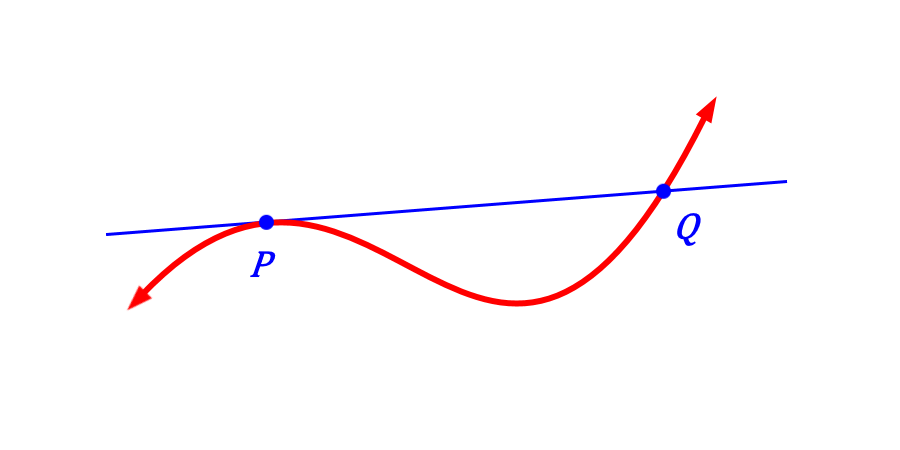
\includegraphics[width=0.35\textwidth]{der_fig1}
\caption*{\textbf{Figura 4.}}
\label{figu:mesh1}
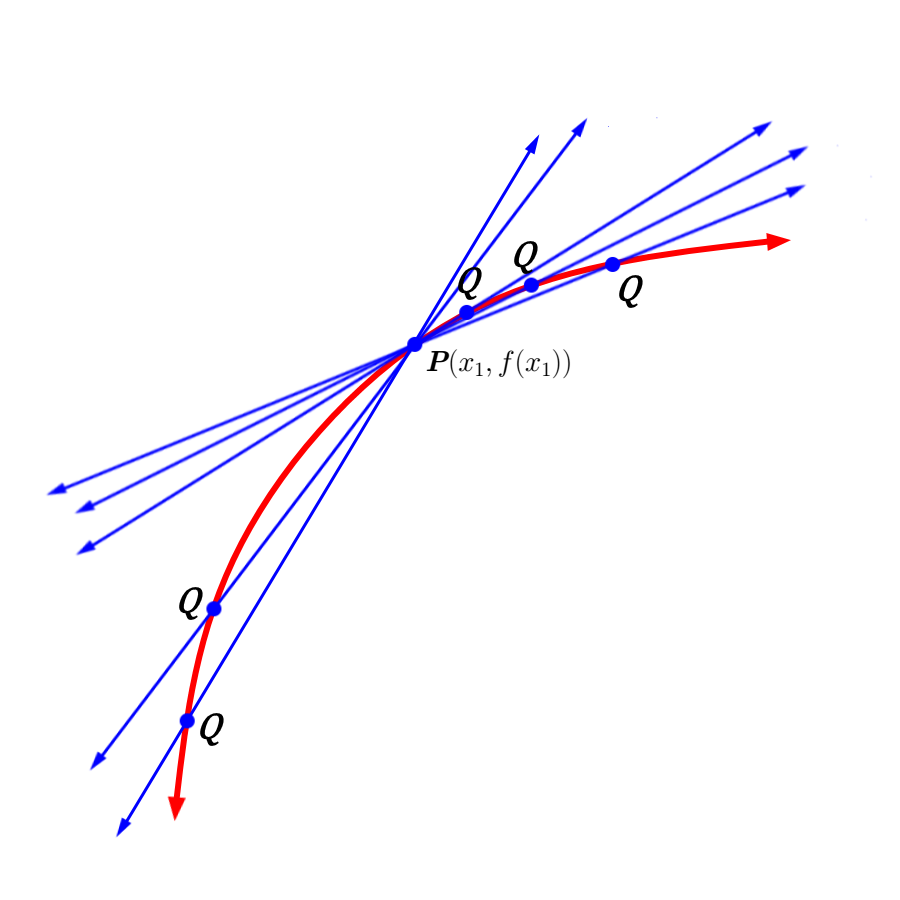
\includegraphics[width=0.35\textwidth]{der_fig2}
\caption*{\textbf{Figura 5.}}
\label{figu:mesh2}
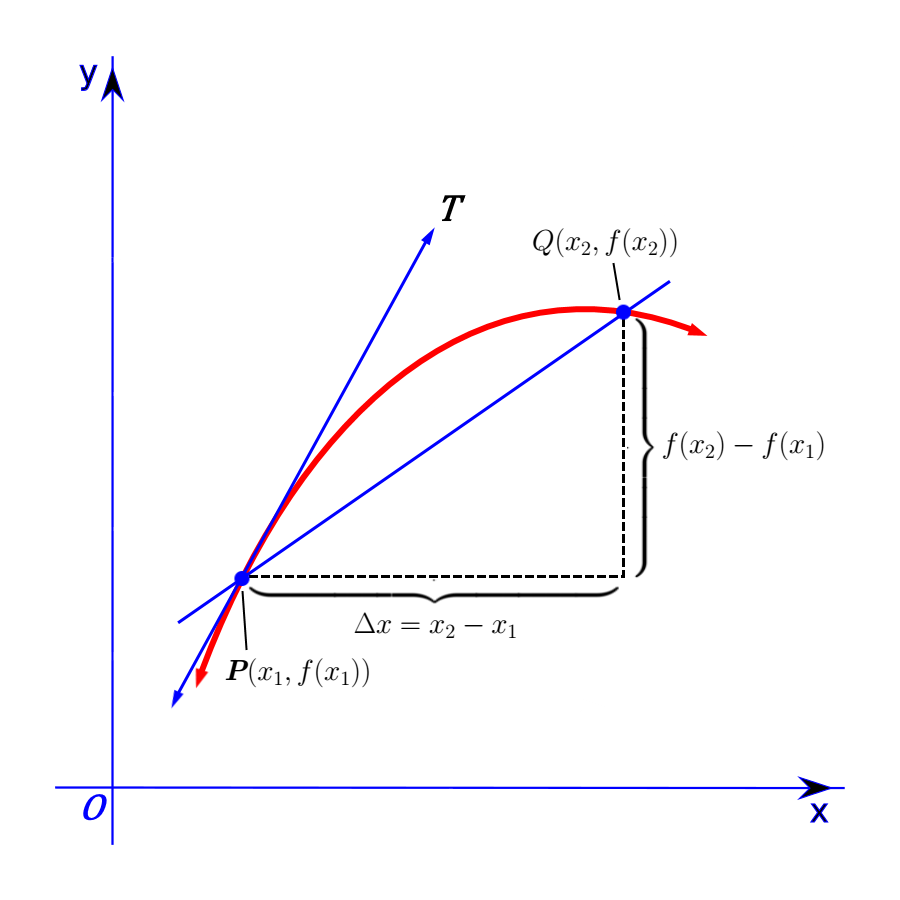
\includegraphics[width=0.35\textwidth]{der_fig3}
\caption*{\textbf{Figura 6.}}
\label{figu:mesh3}
\end{wrapfigure}

\hspace*{10mm}En el cálculo muchos problemas de gran peso dependen de que podamos determinar la recta tangente a la gráfica de una función en un punto específico de su gráfica. La recta tangente en un punto de una circunferencia se define como la recta que intersecta a la circunferencia en un solo punto. En la \textbf{Figura 4} la recta tangente que deberia ser la tangente al punto \textbf{\textit{P}} intersecta a la recta en otro punto \textbf{\textit{Q}}. Para obtener una definición adecuada de la recta tangente, se emplea el concepto de límite a fin definir la pendiente de una recta tangente en el punto. Después, la recta tangente se determina por medio de su pendiente y punto de tangencia.\\
\hspace*{10mm}Considere que la función $f$ es continua en $x_1$. Se desea  definir la pendiente de la recta tangente a la gráfica de $f$ en el punto $P'(x_1,f(x_1))$. Sea $l$ un intervalo abierto que contiene a $x_1$, en el cual está definida $f$. Sea $Q(x_2,f(x_2))$ otro punto sobre la gráfica de $f$ tal que $x_2$ tambien esté en $l$. Dibuje la recta que pasa por \textit{P} y \textit{Q}. Cualquier recta que pase por dos puntos de una curva se denomina \textbf{recta secante}; por tanto, la recta que pasa por \textit{P} y \textit{Q} es una recta secante. En la \textbf{Figura 5}  se muestra la recta secante para varios valores de $x_2$. La \textbf{Figura 6} muestra una recta secante particular. En esta figura \textit{Q} está a la derecha de \textit{P}. Sin embargo, \textit{Q} puede estar a la derecha o a la izquierda de \textit{P}, como se muestra en la figura 5.\\
\hspace*{10mm}La diferencia de las abscisas (las coordenadas $x$) de \textit{Q} y \textit{P} se denota por $\Delta x$ (y se lee "delta $x$") de modo que
$$\Delta x=x_2-x_1$$

\hspace*{10mm}Observe que $\Delta x$ representa el cambio en el valor de $x$ de $x_1$ a $x_2$ y puede ser positivo o negativo. Este cambio recibe el nombre de \textbf{incremento de x}. Note que el símbolo $\Delta x$ para el incremento de $x$ no significa "delta multiplicado por $x$".\\
\hspace*{10mm}Considere la recta secante \textit{PQ} de la figura 6; su pendiente está determinada por
$$m_{PQ}=\frac{f(x_2)-f(x_1)}{\Delta x}$$
\hspace*{10mm}Como $x_2=x_1+\Delta x$, la ecuación anterior puede escribirse como
$$m_{PQ}=\frac{f(x_1+\Delta x)-f(x_1)}{\Delta x}$$

\hspace*{10mm}Ahora considere el  punto \textit{P} como un punto fijo y que el punto \textit{Q} se mueve a lo largo de la curva hacia \textit{P}; esto es, \textit{Q} tiende o se aproxima a \textit{P}. Esto equivale a decir que $\Delta x$ tiende a cero.\\
\begin{wrapfigure}{1}{0.35\textwidth}
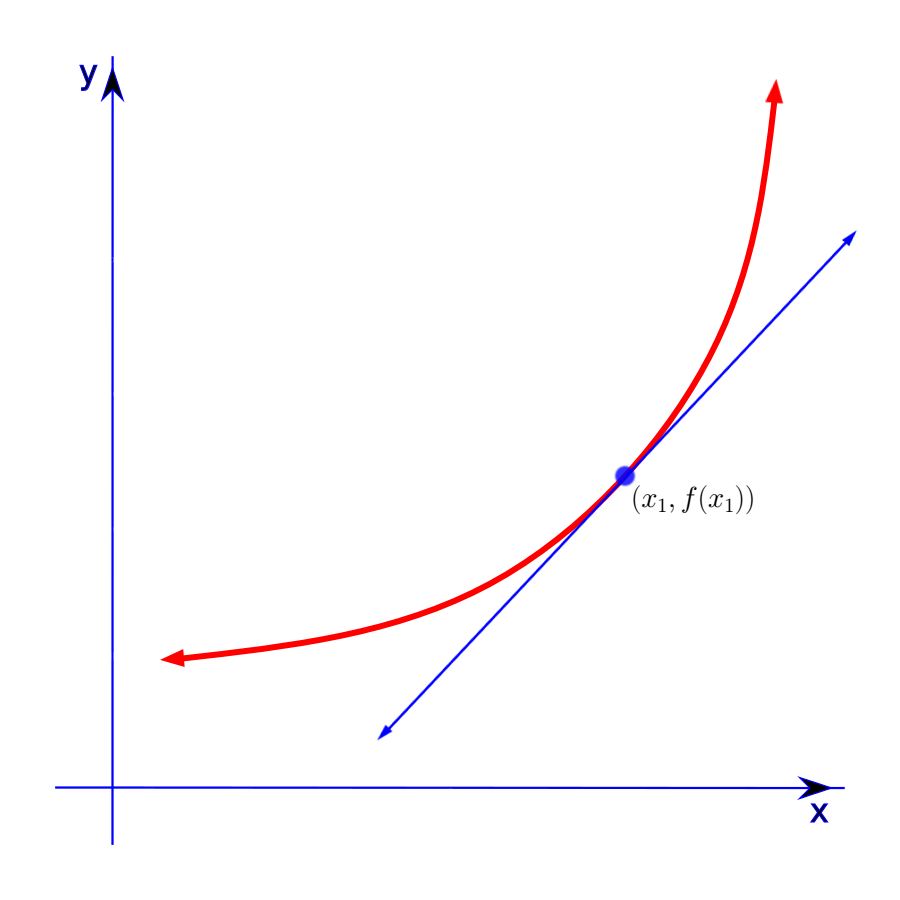
\includegraphics[width=0.35\textwidth]{der_fig4}
\caption*{\textbf{Figura 7.}}
\label{figu:mesh4}
%\end{wrapfigure}
%\begin{wrapfigure}{1}{0.35\textwidth}
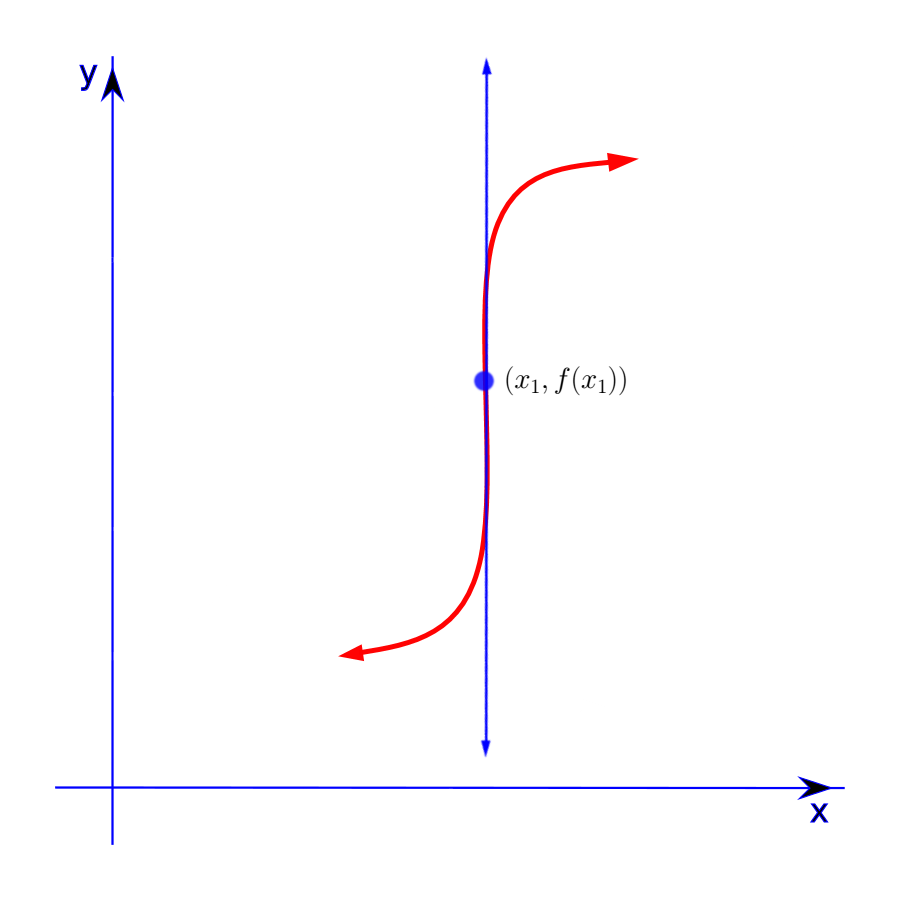
\includegraphics[width=0.35\textwidth]{der_fig5}
\caption*{\textbf{Figura 8.}}
\label{figu:mesh5}
\end{wrapfigure}
\hspace*{10mm}Conforme esto sucede, la recta secante gira sobre el punto fijo \textit{P}. Si la recta secante \textit{PQ} tiene una posición límite, es esta posición límite la que se quiere como la recta tangente a la gráfica de $f$ en el punto \textit{P}. Se desea así, que la pendiente de la recta tangente a la gráfica de $f$ en \textit{P} sea el límite de $m_{PQ}$ conforme $\Delta x$ tiende a cero, si este límite existe. Si $\lim_{\Delta x \to 0}m_{PQ}$ es igual a $+\infty$ o a $-\infty$, entonces conforme $\Delta x$ tiende a cero la recta \textit{PQ} tiende a la recta que pasa por \textit{P} y es paralela al eje $y$. En este caso se desearía que la recta tangente sea la recta $x=x_1$. Esta discusión conduce a la siguiente definición.

Suponga que la función $f$ es continua en $x_1$. La recta tangente a la gráfica de $f$ en el punto \textit{P}$(x_1,f(x_1))$ es\\[2mm]
\textbf{(i)} la recta que pasa por \textit{P} y tiene pendiente $m(x_1)$, dada por

$$m(x_1)= \lim_{\Delta x \to 0} \frac{f(x_1+\Delta x)-f(x_1)}{\Delta x}$$

si este límite existe.\\[2mm]
\textbf{(ii)} la recta $x=x_1$ si
$$\lim_{\Delta x \to 0^+}\frac{f(x_1+\Delta x)-f(x_1)}{\Delta x}\text{ es }+\infty\text{ o }-\infty$$
\hspace*{30mm}y
$$\lim_{\Delta x \to 0^-}\frac{f(x_1+\Delta x)-f(x_1)}{\Delta x}\text{ es }+\infty\text{ o }-\infty$$

\hspace*{10mm}La \textbf{Figura 7} muestra la gráfica de unafunción $f$ y su recta tangente cuando $m(x_1)$ existe. La \textbf{Figura 8} muestra la gráfica de una función $f$ con una recta tangente vertical en el punto $(x_1,f(x_1))$.\\[2mm]
\hspace*{10mm}Si no se cumple ninguno de los incisos anteriores, entonces no existe la recta tangente a la gráfica de $f$ en el punto \textit{P}$(x_1,f(x_1))$.\\[2mm]
\hspace*{10mm}La \textit{pendiente de la recta tangente a la gráfica de una función} en un punto se denomina \textbf{pendiente de la gráfica} en el punto.\\[2mm]
\textbf{Ejemplos.}

1) $\lim_{x\to 0} (3x+2)$
$$f(x)=3x+2$$
$$f(x+\Delta x)=3(x+\Delta x)+2$$
Utilizando la formula de la derivada obtenemos:
$$\lim_{\Delta x \to 0}\frac{f(x+\Delta x)-f(x)}{\Delta x}$$
$$\lim_{\Delta x \to 0}\frac{3(x+\Delta x)+2-(3x+2)}{\Delta x}$$
$$\lim_{\Delta x \to 0}\frac{3x+3\Delta x+2-3x-2}{\Delta x}$$
$$\lim_{\Delta x \to 0}\frac{3x+3\Delta x+2-3x-2}{\Delta x}$$
$$\lim_{\Delta x \to 0}\frac{3\Delta x+\cancel{3x+2}-\cancel{3x-2}}{\Delta x}$$
$$\lim_{\Delta x \to 0}\frac{3\Delta x}{\Delta x}$$
$$\lim_{\Delta x \to 0}\frac{3\cancel{\Delta x}}{\cancel{\Delta x}}$$
$$=3$$

\pagebreak 2) $\lim_{x\to 0} 2x^2-3x+5$
$$f(x+\Delta x)=2(x+\Delta x)^2-3(x+\Delta x)+5$$
Sustituimos en la formula de la derivada:
$$\lim_{\Delta x \to 0}\frac{2(x+\Delta x)^2-3(x+\Delta x)+5-(2x^2-3x+5)}{\Delta x}$$
$$\lim_{\Delta x \to 0}\frac{2(x^2+x\Delta x+x\Delta x+\Delta x^2)\cancel{-3x}-3\Delta x\cancel{+5}-2x^2\cancel{+3x}\cancel{-5}}{\Delta x}$$
$$\lim_{\Delta x \to 0}\frac{\cancel{2x^2}+2x\Delta x+2x\Delta x+2\Delta x^2-3\Delta x\cancel{-2x^2}}{\Delta x}$$
$$\lim_{\Delta x \to 0}\frac{4x\Delta x+2\Delta x^2-3\Delta x}{\Delta x}$$
$$\lim_{\Delta x \to 0}\frac{\cancel{\Delta x}(4x+2\Delta x-3)}{\cancel{\Delta x}}$$
$$\lim_{\Delta x \to 0}4x+2\Delta x -3$$
Evaluamos $\lim_{\Delta x \to 0}$
$$4x+2(0)-3$$
$$=4x-3$$


3) $\lim_{\Delta x \to 0} 3x^2+2x+5$
$$f(x+\Delta x)=3(x+\Delta x)^2+2(x+\Delta x)+5$$
$$\lim_{\Delta x \to 0}\frac{3(x+\Delta x)^2+2(x+\Delta x)+5-(3x^2+2x+5)}{\Delta x}$$
$$\lim_{\Delta x \to 0}\frac{3(x^2+x\Delta x+x\Delta x+\Delta x^2)+2x+2\Delta x+5-3x^2-2x-5}{\Delta x}$$
$$\lim_{\Delta x \to 0}\frac{\cancel{3x^2}+3x\Delta x+3x\Delta x+3\Delta x^2\cancel{+2x}+2\Delta x\cancel{+5}\cancel{-3x^2}\cancel{-2x}\cancel{-5}}{\Delta x}$$
$$\lim_{\Delta x \to 0}\frac{6x\Delta x+3\Delta x^2+2\Delta x}{\Delta x}$$
$$\lim_{\Delta x \to 0}\frac{\cancel{\Delta x}(6x+3\Delta x+2)}{\cancel{\Delta x}}$$
$$\lim_{\Delta x \to 0}6x+3\Delta x+2$$
Evaluamos $\lim_{\Delta x \to 0}$
$$6x+3(0)+2$$
$$=6x+2$$

4) $\lim_{\Delta x \to 0} 6x^3-2x^2+x-10$
$$f(x+\Delta x)=6(x+\Delta x)^3-2(x+\Delta x)^2+(x+\Delta x)-10$$
$$\lim_{\Delta x \to 0}\frac{6(x+\Delta x)^3-2(x+\Delta x)^2+(x+\Delta x)-10-(6x^3-2x^2+x-10)}{\Delta x}$$
$$\lim_{\Delta x \to 0}\frac{6(x^3+3x^2\Delta x+3x\Delta x^2+\Delta x^3)-2(x^2+2x\Delta x+\Delta x^2)+(x+\Delta x)-10-(6x^3-2x^2+x-10)}{\Delta x}$$
$$\lim_{\Delta x \to 0}\frac{6x^3+18x^2\Delta x+18x\Delta x^2+6\Delta x^3-2x^2-4x\Delta x-2\Delta x^2+x+\Delta x-10-6x^3+2x^2-x+10}{\Delta x}$$
$$\lim_{\Delta x \to 0}\frac{\cancel{6x^3}+18x^2\Delta x+18x\Delta x^2+6\Delta x^3\cancel{-2x^2}-4x\Delta x-2\Delta x^2\cancel{+x}+\Delta x\cancel{-10-6x^3+2x^2-x+10}}{\Delta x}$$
$$\lim_{\Delta x \to 0}\frac{18x^2\Delta x+18x\Delta x^2+6\Delta x^3-4x\Delta x-2\Delta x^2+\Delta x}{\Delta x}$$
$$\lim_{\Delta x \to 0}\frac{\cancel{\Delta x}(18x^2+18x\Delta x+6\Delta x^2-4x-2\Delta x+1)}{\cancel{\Delta x}}$$
$$\lim_{\Delta x \to 0}18x^2+18x\Delta x+6\Delta x^2-4x-2\Delta x+1$$
Evaluamos $\lim_{\Delta x \to 0}$
$$18x^2+18x(0)+6(0)^2-4x-2(0)+1$$
$$=18x^2-4x+1$$

5) $\lim_{\Delta x \to 0} x^2-x+2$
$$f(x+\Delta x)=(x+\Delta x)^2-(x+\Delta x)+2$$
$$\lim_{\Delta x \to 0}\frac{(x+\Delta x)^2-(x+\Delta x)+2-(x^2-x+2)}{\Delta x}$$
$$\lim_{\Delta x \to 0}\frac{x^2+2x\Delta x +\Delta x^2-x-\Delta x+2-x^2+x-2)}{\Delta x}$$
$$\lim_{\Delta x \to 0}\frac{\cancel{x^2}+2x\Delta x +\Delta x^2\cancel{-x}-\Delta x\cancel{+2-x^2+x-2}}{\Delta x}$$
$$\lim_{\Delta x \to 0}\frac{2x\Delta x +\Delta x^2-\Delta x}{\Delta x}$$
$$\lim_{\Delta x \to 0}\frac{\cancel{\Delta x}(2x+\Delta x-1)}{\cancel{\Delta x}}$$
$$\lim_{\Delta x \to 0}2x+\Delta x-1$$
Evaluamos $\lim_{\Delta x \to 0}$
$$2x+(0)-1$$
$$=2x-1$$

%------------------------------------LA DERIVADA-------------------------------
%---------------------------------------LEYES----------------------------------
\pagebreak \textbf{Leyes de la derivada.}\\[2mm]
\textbf{1)}\textit{La derivada de una constante es 0:}
$$f(x)=k\Longrightarrow f'(x)=0$$
Ejemplo:
$$f(x)=-3 \Longrightarrow f'(x)=0$$
\textbf{2)}\textit{La derivada de una función identidad es 1:}
$$f(x)=x \Longrightarrow f'(x)=1$$
\textbf{3)}\textit{La derivada de $x$ elevado a un numero real $n$ es el producto de ese número real por $x$ elevado a ese mismo número menos una unidad:}
$$f(x)=x^n \Longrightarrow f'(x)=n\cdot x^{n-1}\forall n \in \R$$
Ejemplo:
$$f(x)=x^3 \Longrightarrow f'(x)=3\cdot x^{3-1}=3x^2$$
\textbf{4)}\textit{La derivada de la multiplicación de un numero real $k$ por una función es el numero real por la derivada de la función:}
$$k\cdot x^n \Longrightarrow f'(x)=k\cdot n\cdot x^{n-1}$$
Ejemplo:
$$f(x)=4x^2 \Longrightarrow f'(x)=4\cdot 2\cdot x^{2-1}=8x$$
\textbf{5)}\textit{La derivada de un radical viene dada por:}
$$f(x)=\sqrt[n]{x}\Longrightarrow f'(x)=\frac{1}{n\sqrt[n]{x^{n-1}}}$$
$$f(x)=\sqrt{x} \Longrightarrow f'(x)=\frac{1}{2\sqrt{x}}$$
Ejemplo:
$$f(x)=\sqrt{x} \Longrightarrow f'(x)=\frac{1}{2\sqrt{x}}$$
$$f(x)=\sqrt[3]{x} \Longrightarrow f'(x)=\frac{1}{3\sqrt{x^2}}$$
\textbf{6)}\textit{La derivada del logaritmo natural es:}
$$f(x)=\ln(x) \Longrightarrow f'(x)=\frac{1}{x}$$
Ejemplo:
$$f(x)=3\cdot \ln(x) \Longrightarrow f'(x)=3\cdot \frac{1}{x}$$
\textbf{7)}\textit{La derivada del logaritmo en base a es:}
$$f(x)=\log_a(x) \Longrightarrow f'(x)=\frac{1}{x}\log_a(e) \quad \text{Siendo }a \in \R^+$$
Ejemplo:
$$f(x)=3\cdot \log_2(x) \Longrightarrow f'(x)=3\cdot \frac{1}{x}\log_2(e)$$
\textbf{8)}\textit{La derivada de e elevado a x es e elevado a x:}
$$f(x)=e^x \Longrightarrow f'(x)=3e^x$$
$$f(x)=e^x \Longrightarrow f'(x)=-e^x$$
\textbf{9)}\textit{La derivada de la función exponencial a elevado a x, siendo a cualquier numaro real positivo es:}
$$f(x)=a^x \Longrightarrow a^x\cdot \ln(a)$$
Ejemplo
$$f(x)=3^x \Longrightarrow f'(x)=3^x\cdot \ln(3)$$
$$f(x)=e^x \Longrightarrow f'(x)=e^x\cdot \ln(e)=e^x$$
\textbf{10)}\textit{La derivada del seno es el coseno:}
$$f(x)= \sin(x) \Longrightarrow \cos(x)$$
Ejemplo:
$$3\cdot \sin(x) \Longrightarrow f'(x)=3\cdot \cos(x)$$
\textbf{11)}\textit{La derivada del coseno es el seno, con signo negativo:}
$$f(x)=\cos(x) \Longrightarrow f'(x)=-\sin(x)$$
Ejemplo:
$$f(x)=3\cdot \cos(x) \Longrightarrow f'(x)=-3\cdot \sin(x)$$
\textbf{12)}\textit{La derivada de la tangente puede ser escrita de las tres maneras equivalentes:}
$$f(x)=\tan(x) \Longrightarrow f'(x)=\frac{1}{\cos^2(x)}=1+\tan^2(x)=\sec^2(x)$$
Ejemplo:
$$f(x)=2\cdot \tan(x) \Longrightarrow f'(x)=\frac{2}{\cos^2(x)}$$
\textbf{13)}\textit{La derivada del arcoseno es:}
$$f(x)=\arcsin(x) \Longrightarrow f'(x)=\frac{1}{\sqrt{1-x^2}}$$
Ejemplo:
$$f(x)=3\cdot \arcsin(x) \Longrightarrow f'(x)=3\cdot \frac{1}{1-x^2}$$
\textbf{14)}\textit{La derivada del arcocoseno es:}
$$f(x)=\arccos(x) \Longrightarrow f'(x)=\frac{-1}{\sqrt{1-x^2}}$$
Ejemplo:
$$f(x)=-3\cdot \arccos(x) \Longrightarrow f'(x)-3\cdot \frac{-1}{\sqrt{1-x^2}}=\frac{3}{\sqrt{1-x^2}}$$
\textbf{15)}\textit{La derivada del arcotangente es:}
$$f(x)=\arctan(x) \Longrightarrow f'(x)=\frac{1}{1+x^2}$$
Ejemplo:
$$f(x)=\frac{1}{4}\cdot \arctan(x) \Longrightarrow f'(x)=\frac{1}{4}\cdot \frac{1}{1+x^2}$$

\pagebreak \textbf{Derivada de la suma y resta de funciones.}\\[2mm]
\textit{La derivada de la suma de varias funciones es la suma de sus derivadas. La derivada de la resta de varias funciones es la resta de sus derivadas. Por tanto, para cualquier valor de x en que dos funciones f y g sean derivables, se cumple:}
$$D(f+g)=f'+g';\quad D(f-g)=f'-g'$$
Ejemplo:
\begin{center}
\begin{tabular}{ccc}
$f(x)3x^2$ & &$D(f+g)=D(3x^2+2x)=D(3x^2)+D(2x)=6x+2$\\
 &$\Longrightarrow$ &  \\
$g(x)=2x$ & &$D(f-g)=D(3x^2-2x)=D(3x^2)-D(2x)=6x-2$\\
\end{tabular}
\end{center}

\textbf{Derivada del producto.}\\[2mm]
\textit{La derivada del producto de dos funciones es igual a la derivada de la primera función por la segunda sin derivar, más la derivada de la segunda función por la primera sin derivar. Por tanto, para cualquier valor de x en que dos funciones f y g sean derivables, se cumple:}
$$D(f\cdot g)=f'\cdot g+f\cdot g'$$
Ejemplo:
\begin{center}
\begin{tabular}{ccccc}
$f(x)3x^2$ & &$f'(x)=6x$& & \multirow{3}{*}{$D(f\cdot g)=6x\cdot \ln(x)+3x^2\cdot \frac{1}{x}$}\\
 &$\Longrightarrow$ & & $\Longrightarrow$ &  \\
$g(x)=\ln(x)$ & &$g'(x)=\frac{1}{x}$& & \\
\end{tabular}
\end{center}

\textbf{Derivada del cociente.}\\[2mm]
\textit{La derivada del cociente de dos funciones es igual a la derivada de la primera función por la segunda sin derivar, menos la derivada de la segunda función por la primera sin derivar, dividido todo ello por la segunda función al cuadrado. Por tanto, para cualquier valor de x en que dos funciones f y g sean derivables, y que g sea distinto de cero, se cumple:}
$$D\left(\frac{f}{g}\right)=\frac{f'\cdot g-f\cdot g'}{g^2}$$
Ejemplo:
\begin{center}
\begin{table}[h]
\begin{tabular}{ccccc}
$f(x)3x^2$ & &$f'(x)=6x$& & \multirow{3}{*}{$D\left(\frac{f}{g}\right)=\frac{6x\cdot \ln(x)-3x^2\cdot \frac{1}{x}}{\ln^2(x)}=\frac{3x\cdot (2\cdot \ln(x)-1)}{\ln^2(x)}$}\\
 &$\Longrightarrow$ & & $\Longrightarrow$ &  \\
$g(x)=\ln(x)$ & &$g'(x)=\frac{1}{x}$& & \\
\end{tabular}
\end{table}
\end{center}

\textbf{Derivada de la composición.}\\[2mm]
\textit{La derivada de la composición de funciones también se conoce como regla de la cadena y establece que si f es derivable en x y g lo es en f(x), g$\circ$f será derivable en x y tendrá por expresión:}
$$D[(g \circ f)(x)]=D[g(f(x))]=g'(f(x))\cdot f'(x)$$
Ejemplo:
$$f(x)=\underbrace{(\sin(x))^2}_{g(x)}\Longrightarrow f'(x)=2(\sin(x))^{2-1}\cdot \underbrace{cos(x)}_{g'(x)}=2\sin(x) \cos(x)$$
$$f(x)=\ln \underbrace{(x^2)}_{g(x)} \Longrightarrow f'(x)=\frac{1}{x^2}\cdot \underbrace{2x}_{g'(x)}=\frac{2}{x}$$

%------------------------------------LA DERIVADA-------------------------------
%------------------------------------EJERCICIOS--------------------------------
\pagebreak 1) $y=4+2x+3x^2-5x^3-8x^4-9x^5$
$$=\cancelto{0}{\dx (4)}+2\left(\dx (x)\right)+3\left(\dx (x^2)\right)-5\left(\dx (x^3)\right)-8\left(\dx (x^4)\right)-9\left(\dx (x^5)\right)$$
$$=\cancelto{1}{2\left(\dx (x)\right)}+3\left(\dx (x^2)\right)-5\left(\dx (x^3)\right)-8\left(\dx (x^4)\right)-9\left(\dx (x^5)\right)$$
$$\text{Usamos la regla de la potencia, }\dx (x^n)=n x^{n-1}$$ 
$$=2(1)+3(2x)-5\left(\dx (x^3)\right)-8\left(\dx (x^4)\right)-9\left(\dx (x^5)\right)$$
$$=2+6x-5(3x^2)-8\left(\dx (x^4)\right)-9\left(\dx (x^5)\right)$$
$$=2+6x-15x^2-8(4x^3)-9\left(\dx (x^5)\right)$$
$$=2+6x-15x^2-32x^3-9(5x^4)$$
$$=2+6x-15x^2-32x^3-45x^4$$

2) $y=\dfrac{1}{x}+\dfrac{3}{x^2}+\dfrac{2}{x^3}$
$$=\dx \left(\frac{1}{x}\right) + 3\left(\dx \left(\frac{1}{x^2}\right)\right) + 2 \left(\dx \left(\frac{1}{x^3}\right)\right)$$
$$\text{Usamos la regla de la potencia, }\dx (x^n)=n x^{n-1}\text{, donde }\dx\left(\frac{1}{x}\right)=\dx (x^{-1})=-x^{-2} $$ 
$$=-\frac{1}{x^2} + 3\left(\dx \left(\frac{1}{x^2}\right)\right) + 2 \left(\dx \left(\frac{1}{x^3}\right)\right)$$
$$=-\frac{1}{x^2} + 3\left( -\frac{2}{x^3} \right) + 2 \left(\dx \left(\frac{1}{x^3}\right)\right)$$
$$=-\frac{1}{x^2} + -\frac{6}{x^3} + 2 \left( -\frac{3}{x^4} \right)$$
$$=-\frac{1}{x^2} + -\frac{6}{x^3} -\frac{6}{x^4}$$

3) $y=2x^{1/2}+6x^{1/3}-2x^{3/2}$
$$=2\left( \dx \left( x^{1/2} \right) \right) + 6\left( \dx \left( x^{1/3} \right) \right) -2 \left( \dx \left( x^{3/2} \right) \right)$$
$$\text{Usamos la regla de la potencia, }\dx (x^n)=n x^{n-1}$$ 
$$=2\left( \frac{1}{2}\cdot x^{-1/2} \right)+ 6\left( \dx \left( x^{1/3} \right) \right) -2 \left( \dx \left( x^{3/2} \right) \right)$$
$$=2\left( \frac{1}{2}\cdot \frac{1}{\sqrt{x}} \right)+ 6\left( \frac{x^{-2/3}}{3} \right) -2 \left( \dx \left( x^{3/2} \right) \right)$$
$$=2\left( \frac{1}{2\sqrt{x}} \right)+ 6\left( \frac{1}{3x^{2/3}} \right) -2 \left( \frac{3\sqrt{x}}{2} \right)$$
$$=\frac{1}{\sqrt{x}} + \frac{2}{x^{2/3}} -3\sqrt{x}$$

\pagebreak 4) $y=\sqrt[3]{x^2}-\dfrac{1}{\sqrt{5x}}$
$$=\dx \left(\sqrt[3]{x^2}\right) +\dx \left( -\dfrac{1}{\sqrt{5x}} \right)$$
$$\text{Usamos la regla de la cadena, }\dx \left(\sqrt[3]{x^2}\right)=\frac{d\sqrt[3]{u}}{du}\frac{du}{dx}\text{, donde }u=x^2 \text{ y } \frac{d}{du}\left( \sqrt[3]{u} \right) = \frac{1}{3u^{2/3}}$$
$$=\frac{\dx (x^2)}{3(x^2)^{2/3}} +\dx \left( -\dfrac{1}{\sqrt{5x}} \right)$$
$$=\frac{2x}{3(x^2)^{2/3}} +\dx \left( -\dfrac{1}{\sqrt{5x}} \right)$$
$$=\frac{2x}{3(x^2)^{2/3}} +\dx \left( -\dfrac{1}{\sqrt{5}}\cdot \frac{1}{\sqrt{x}} \right)$$
$$=\frac{2x}{3(x^2)^{2/3}} -\dfrac{1}{\sqrt{5}}\left( \dx \left( \frac{1}{\sqrt{x}} \right) \right)$$
$$\text{Usamos la regla de la potencia, }\dx (x^n)=n x^{n-1}\text{ donde }n=-\frac{1}{2}\quad \dx \left(\frac{1}{\sqrt{x}}\right)=\dx (x^{-1/2})=-\frac{1}{2}x^{-3/2}$$ 
$$=\frac{2x}{3(x^2)^{2/3}} -\dfrac{1}{\sqrt{5}}\left(-\frac{1}{2}x^{-3/2}\right)$$
$$=\frac{2x}{3(x^2)^{2/3}} +\dfrac{1}{\sqrt{5}}\left(-\frac{1}{2x^{3/2}}\right)$$
$$=\frac{2x}{3(x^2)^{2/3}} +\dfrac{1}{\sqrt{5}\cdot 2x^{3/2}}$$

5) $y=(t^2-3)^4$
$$\dt \left( (t^2-3)^4 \right)$$
$$\text{Usando la regla de la cadena, }\frac{du^4}{du}\frac{du}{dt}\text{, donde }u=t^2-3 \text{ y }\frac{d}{du}(u^4)=4u^3$$
$$=4(-3+t^2)^3\left(\dx (-3+t^2)\right)$$
$$=4(-3+t^2)^3\left( \cancelto{0}{\dx (-3)}+\dx (t^2) \right)$$
$$\text{Usamos la regla de la potencia, }\dx (t^2)=2 x^{2-1}= 2t$$ 
$$=4(-3+t^2)^3(2t)$$
$$=8(-3+t^2)^3$$

%------------------------------------LA ANTIDERIVADA---------------------------
%------------------------------------------------------------------------------
\pagebreak \textbf {La Antiderivada}\\[2mm]
\hspace*{10mm}La \textit{antiderivación} o \text{antidiferenciación}, es la opereción inversa a la derivada y es el proceso mediante el cual se determina el conjunto de todas las antiderivadas de una función dada. El símbolo $\int_{}^{}$ denota la operación de antiderivación, y se escribe
$$\int_{}^{}f(x)\, dx=F(x)+C$$
\hspace*{50mm}donde
$$F'(x)=f(x)$$
\hspace*{50mm}y
$$d(F(x))=f(x)dx$$
La expresion $F(x)+C$ recibe el nombre de \textbf{antiderivada general} de $f$.\\[2mm]
\hspace*{10mm}Leibniz introdujo la convención de escribir la diferencial de una función antes del símbolo de antiderivación y se puede escribir:
$$\int_{}^{}d(f(x))=F(x)+C$$
Esta ecuación establece que cuando se antideriva la diferencial de una función, se obtiene esa función más una constante arbitraria. De este modo puede considerarse que el símbolo para antiderivación representa la operación inversa a la operación denotada por $d$ para calcular una diferencial.\\[2mm]
\hspace*{10mm}Si ${F(x)+C}$ es el conjunto de todas las funciones cuyas diferenciales son $f(x)dx$, también es el conjunto de todas las funciones cuya derivada es $f(x)$. Por tanto, la antiderivación se considera como la \textit{operación para determinar el conjunto de todas las funciones que tienen una derivada dada}.\\[2mm]
\hspace*{10mm}Como la antiderivación es la operación inversa de la derivación, los teoremas  de antiderivación se obtienen de los teoremas de diferenciación. Así los teoremas siguientes pueden demostrarse a partir de los teoremas correspondientes de diferenciación.\\[2mm]
\hspace*{10mm}1.$\quad\displaystyle\int dx=x+C$\\[2mm]
\hspace*{10mm}2.$\quad\displaystyle\int af(x) dx=a\int f(x) dx\quad$donde $a$ es una constante\\[2mm]
\hspace*{10mm}El teorema 2 establece que la antiderivada general del producto de una constante por una función es la constante por la antiderivada general de la función.\\[2mm]
\hspace*{10mm}3.$\quad\displaystyle\int [f(x)+g(x)]dx=\int f(x)dx + \int g(x)dx$\\[2mm]
\hspace*{10mm}El teorema 3 establece que la antiderivada general de la suma de dos funciones es igual a la suma de las antiderivadas generales de las funciones, considerando que ambas funciones están definidas en el mismo intervalo. Al extender el teorema 3 para un numero finito de funciones y combinándolo con el teorema 2, se obtiene el teorema siguiente.\\[2mm]
\hspace*{10mm}4.$\quad\text{Si $f_1,f_2,...,f_n$ están definidas en el mismo intervalo, entonces}$\\[2mm]
\hspace*{12mm}$\quad\displaystyle\int [c_1f_1(x)+c_2f_2(x)+...+c_nf_n(x)]dx$\\[2mm]
\hspace*{22mm}$=c_1\displaystyle\int f_1(x)dx+c_2\int f_2(x)dx+...+c_n\int f_n(x)dx\quad$donde $c_1,c_2,...c_n$ son constantes\\[2mm]
\hspace*{10mm}5.$\quad\displaystyle\int x^ndx=\frac{x^{n+1}}{n+1}+C\quad n\neq -1$\\[2mm]
\textbf{Ejemplos.}\\[2mm]
1) $\displaystyle\int x^6dx$
$$=\frac{x^{6+1}}{6+1}+C$$
$$=\frac{x^7}{7}+C$$
2) $\displaystyle\int x^{\frac{2}{3}}dx$
$$=\frac{x^{\frac{2}{3}+1}}{\frac{2}{3}+1}+C$$
$$=\frac{x^{\frac{5}{3}}}{\frac{5}{3}}+C$$
3) $\displaystyle\int \sqrt[3]{x}dx$
$$=\int x^{\frac{1}{3}}dx$$
$$=\frac{x^{\frac{1}{3}+1}}{\frac{1}{3}+1}+C$$
$$=\frac{x^{\frac{4}{3}}}{\frac{4}{3}}+C$$
$$=\frac{3}{4}x^{\frac{4}{3}}+C$$
$$=\frac{3}{4}x\sqrt[3]{x}+C$$
4) $\displaystyle\int (x^4-6x^2-2x+4)dx$
$$=\frac{x^5}{5}-\frac{6x^3}{3}-\frac{2x^2}{2}+4x+C$$
$$=\frac{x^5}{5}-2x^3-x^2+4x+C$$
5) $\displaystyle\int \left( \sqrt{5x}+\sqrt{\dfrac{5}{x}} \right) dx$
$$=\int (\sqrt{5}x^{1/2}+\sqrt{5}x^{-1/2})dx$$
$$=\sqrt{5}\frac{x^{3/2}}{\frac{3}{2}}+\sqrt{5}\frac{x^{1/2}}{\frac{1}{2}}+C$$
$$=\frac{2\sqrt{5}x\sqrt{x}}{3}+2\sqrt{5}x\sqrt{x}+C$$
$$=\frac{2x\sqrt{5x}}{3}+2x\sqrt{5x}+C$$

%------------------------------------LA ANTIDERIVADA---------------------------
%-----------------------------------------LEYES--------------------------------
\pagebreak \textbf{Leyes de la antiderivada.}\\[2mm]
\textbf{1)}\textit{La antiderivada o integral de una suma de funciones es igual a la suma de las integrales de esas funciones:}
$$\int [f(x)+g(x)dx] \Longrightarrow \int f(x)dx+\int g(x)dx$$
Ejemplo:
$$\int [x^2+2x dx] \Longrightarrow \int x^2dx+\int 2xdx$$
\textbf{2)}\textit{La integral del producto de una constante por una función es igual a la constante por la integral de la función:}
$$\int kf(x)dx \Longrightarrow k\int f(x)dx$$
Ejemplo:
$$\int 3x^2dx \Longrightarrow 3\int x^2dx$$
\textbf{3)}\textit{La integral de una constante es igual a la constante por la variable $x$:}
$$\int kdx = k\cdot x +C$$
Ejemplo:
$$\int 2dx \Longrightarrow 2x+C$$
\textbf{4)}\textit{La integral de cero es una constante:}
$$\int 0dx = C$$
\textbf{5)}\textit{La integral de una potencia es igual a la variable elevada a la potencia $n+1$ sobre $n+1$ sumando una constante:}
$$\int x^ndx= \frac{x^{n+1}}{n+1}+C$$
$$\int u^n\cdot u'dx=\frac{u^{n+1}}{n+1}+C\quad \neq -1$$
Si \textbf{a, k y C} son constantes; \textbf{u} es una función y \textbf{u'} es la \textbf{derivada} de u, obtenemos las siguientes integrales:\\[2mm]
\begin{multicols}{2}
\hspace*{10mm}$\displaystyle\int \frac{u'}{u}dx=\ln u +C$\\[2mm]
\hspace*{10mm}$\displaystyle\int a^u\cdot u'dx=\frac{a^u}{\ln (a)}+C$\\[2mm]
\hspace*{10mm}$\displaystyle\int e^u\cdot u'dx=e^u+C$\\[2mm]
\hspace*{10mm}$\displaystyle\int \sin u \cdot u'dx = -\cos u +C$\\[2mm]
\hspace*{10mm}$\displaystyle\int \cos u \cdot u'dx = \sin u +C$\\[2mm]
\hspace*{10mm}$\displaystyle\int \frac{u'}{\sqrt{1-u^2}}dx=\arcsin u +C$\\[2mm]
\hspace*{10mm}$\displaystyle\int \frac{u'}{1+u^2}dx=\arctan u +C$\\[2mm]
\end{multicols}
\hspace*{10mm}$\displaystyle\int \frac{u'}{\cos^2u}dx=\int \sec^2u\cdot u'dx=\int (1+ \tan^2u)\cdot u'dx=\tan u +C$\\[2mm]
\hspace*{10mm}$\displaystyle\int \frac{u'}{\sin^2u}\cdot u'dx=\int \csc^2u\cdot u'dx=\int (1+ \cot^2u)\cdot u'dx=-\cot u +C$\\[2mm]

%------------------------------------LA ANTIDERIVADA---------------------------
%--------------------------------------EJERCICIOS------------------------------
\pagebreak \textbf{Ejercicios.}\\[2mm]
\textbf{1)}$\displaystyle \int \sqrt[3]{x}dx$
$$=\int x^{1/3}dx$$
Aplicando la regla de la potencia:
$$=\frac{x^{(1/3)+1}}{\frac{1}{3}+1}+C$$
$$=\frac{3x^{4/3}}{4}+C$$
\textbf{2)}$\displaystyle \int \frac{1}{x^2}dx$
$$=\int x^{-2}dx$$
Aplicando la regla de la potencia:
$$=\frac{x^{-2+1}}{-2+1}+C$$
$$=\frac{x^{-1}}{-1}+C$$
$$=-x^{-1}+C$$
$$=-\frac{1}{x}+C$$
\textbf{3)}$\displaystyle \int 7x^3dx$
$$=7\int x^3 dx$$
Aplicando la regla de la potencia:
$$=7 \left( \frac{x^{3+1}}{3+1}+C \right)+C$$
$$=7 \left( \frac{x^4}{4} \right)+C$$
$$=\frac{7x^4}{4}+C$$
\textbf{4)}$\displaystyle \int (x^2+4)dx$
$$=\int x^2dx+4\int 1dx$$
$$=\frac{x^{2+1}}{2+1}+4(x)+C$$
$$=\frac{x^3}{3}+4x+C$$
\textbf{5)}$\displaystyle \int (3x^6-4x)dx$
$$=3\int x^6dx - 4 \int x dx$$
$$=3\left( \frac{x^7}{7}\right) -4\left( \frac{x^2}{2}\right) +C$$
$$=\frac{3x^7}{7}-2x^2+C$$
\end{document}

